\documentclass[a4paper,11pt]{article}

\usepackage{../../zyancamlec}
\usepackage[compat=1.1.0]{tikz-feynhand}
\usepackage[offset=1.25em]{simpler-wick}
\def\ntripos{Mathematical Tripos}
\def\npart{III}
\def\ncourse{Quantum Field Theory}
\def\nscourse{QFT}
\def\nlecturer{N.\ Dorey}
\def\nterm{Michaelmas}
\def\nyear{2020}


\begin{document}
	\maketitlepage
	\preliminaries

	\section*{Course Information}
	
	\noindent Quantum Field Theory is the marriage of quantum mechanics with special relativity and provides the mathematical framework in which to describe the interactions of elementary particles.

	\noindent This first Quantum Field Theory course introduces the basic types of fields which play an important role in high energy physics: scalar, spinor (Dirac), and vector (gauge) fields. The relativistic invariance and symmetry properties of these fields are discussed using the language of Lagrangians and Noether’s theorem.

	\noindent The quantisation of the basic non-interacting free fields is firstly developed using the Hamiltonian and canonical methods in terms of operators which create and annihilate particles and anti-particles. The associated Fock space of quantum physical states is explained together with ideas about how particles propagate in spacetime and their statistics.

	\noindent Interactions betweeen fields are examined next, using the interaction picture, Dyson’s formula and Wick’s theorem. A ‘short version’ of these techniques is introduced: Feynman diagrams. Decay rates and interaction cross-sections are introduced, along with the associated kinematics and Mandelstam variables.

	\noindent Spinors and the Dirac equation are explored in detail, along with parity and $\gamma^{5}$. Fermionic quantisation is developed, along with Feynman rules and Feynman propagators for fermions.

	\noindent Finally, quantum electrodynamics (QED) is developed. A connection between the field strength tensor and Maxwell’s equations is carefully made, before gauge symmetry is introduced. Lorentz gauge is used as an example, before quantisation of the electromagnetic field and the Gupta-Bleuler condition. The interactions between photons and charged matter is governed by the principal of minimal coupling. Finally, an example QED cross-section calculation is performed.

	\section*{Pre-requisites}

	You will need to be comfortable with the Lagrangian and Hamiltonian formulations of classical mechanics and with special relativity. You will also need to have taken an advanced course on quantum mechanics.

	\newpage

	\section*{Introduction}
	\subsection*{Why do we need QFT?}
	If we consider the description of the interaction between two charged particles, for an accurate prediction, we need 
	\begin{itemize}
		\item \emph{Maxwell's theory} using a field theoretic perspective (using electric field $\vb{E}(\vb x, t)$ and magnetic field $\vb B(\vb x, t)$), which embodies \emph{locality} and encodes \emph{Lorentz invariance};
		\item And \emph{quantum mechanics} as the charged particles are too small to be considered classically. This encodes the \emph{``discrete''} and \emph{probabilistic} nature.
	\end{itemize}

	The reconcile of special relativity and quantum mechanics leads to \emph{Quantum Field Theory}, where new phenomena emerge:
	\begin{itemize}
		\item Particle creation;
		\begin{center}
			\begin{tikzpicture}[baseline=-5pt]
				\begin{feynhand}
					\vertex (i) at (0,0) {$\gamma$};
					\vertex (f1) at (2.5,1) {$e^+$};
					\vertex (f2) at (2.5,-1) {$e^-$};
					\vertex [particle] (a) at (1.5,0);

					\propag [pho] (i) to [] (a);
					\propag [antfer] (a) to [] (f1);
					\propag [fer] (a) to [] (f2);
				\end{feynhand}
			\end{tikzpicture}
			$\quad$ with $\quad E_{\gamma} \geq 2 m_e c^2$
		\end{center}
		\item Bose/Fermi statistics;
		\item And more...
	\end{itemize}

	It is typical to consider experiments where some initial state $\ket{i}$ transitions to $\ket{f}$.
	
	\needfig{1}

	The challenge we are facing is to calculate the probability 
	\[
		P_{i \to f} = \abs{\mathcal{A}_{i \to f}}^2
	\]
	where $A_{i \to f} \in \mathbb{C}$ is the amplitude of such transition.

	The properties of such probability are
	\begin{itemize}
		\item Unitarity: $\sum_f P_{i \to f} = 1$;
		\item Lorentz covariance.
	\end{itemize}

	\subsection*{What is QFT?}
	Instead of QM, we start from classical field theory.

	For a classical field $\phi(\vb x, t)$, we can use \emph{canonical quantisation} analogous to that in particle QM to obtain a quantum field operator $\hat{\phi}(\vb x,t)$. We will mainly follow this route in this course.

	Quantum field operators are very complicated things --- they are operator-valued functions in space and time.

	There are some key facts in QFT:
	\begin{itemize}
		\item Eigenstates of \emph{Hamiltonian} $\hat{H}[\hat{\phi}, \hat{\pi}]$ describes \emph{multi-particle states}. (We can obtain the eigenstates at least in a free field theory);
		\item We can calculate \[
			\mathcal{A}_{i \to f} = \mel{f}{e^{\mathrm{i} \hat{H} T}}{i}.
		\]
	\end{itemize}

	The remarkable feature of field theories is that there are very few which they can be consistently calculated. Thus we are left to limited, confined choices, which is an attractive character QFTs. Among these, \emph{gauge theories} are a special type, using which we can successfully describe our universe to some extent.

	\subsection*{Outline}
	\begin{enumerate}
		\item Classical Field Theory
		\item Free QFT
		\item Interacting QFT
		\item Fermions
		\item QED
	\end{enumerate}

	\newpage
	
	\tableofcontents
	\newpage
	\maintext
	\setcounter{section}{-1}
	\section{Preliminaries}
	\lec{1}
	\subsection{Units}
	In SI units, we know the dimensions of several fundamental constants are
	\begin{align*}
		c & \sim LT^{-1}\\
		\hbar & \sim L^2 M T^{-1}\\
		G & \sim L^3 M^{-1} T^{-2}
	\end{align*}

	In this course, we choose \emph{natural units} such that
	\[
		\hbar = c = 1
	\]
	
	Note that we are eliminating several dimensions identified in SI units, thus all quantities scale with some power of \emph{mass} or \emph{energy}.
	\[
		X \sim M^\delta
	\]
	where we call $\delta$ the dimension of the quantity and write
	\[
		[X] = \delta
	\]
	
	\begin{ex}
		\[
			[E] = +1 \qquad [L] = -1
		\]
	\end{ex}

	\subsection{Relativity}

	Unless otherwise stated, we use Einstein summation convention throughout the course.

	We work in Minkowski spacetime $\mathbb{R}^{3,1}$ with metric tensor
	\[
		\eta_{\mu\nu} = \diag \{+1, -1, -1, -1\}
	\]
	with the above conventional signature.

	We denote the coordinates in spacetime as 
	\[
		x^\mu = (t, \vb x)
	\]
	and using the metric, we have
	\[
		x_\mu = \eta_{\mu\nu} x^\nu
	\]
	known as ``lowering'' the indices. 
	
	Similarly, for ``raising'' the indices we use the inverse metric tensor $\eta^{\mu\nu}$ defined by
	\[
		\eta^{\mu\nu} \eta_{\nu\rho} = \delta^\mu_\rho
	\]
	\newpage
	\section{Classical Field Theory}

	\subsection{Lorentz Covariant Fields}

	Firstly, let's recall that the Minkowski metric is invariant under Lorentz transformations. And we consider the Lorentz transformation of coordinates:
	\begin{equation}
		x^\mu \mapsto (x')^\mu = \LT{\mu}{\nu}x^\nu
	\end{equation}
	where $\LT{\mu}{\nu}$ is a $4\times 4$ matrix encoding the Lorentz transformation. To find the properties of such $\Lambda$, we write
	\begin{equation}
		\LT{\mu}{\sigma}\LT{\nu}{\tau} \eta^{\sigma\tau} = \eta^{\mu\nu}
	\end{equation}

	Also, we exclude the time-reversal transformations by imposing
	\[
		\det \Lambda = + 1
	\]
	
	The conditions above fix \emph{proper} Lorentz transformations. These have 6 degrees of freedom: 3 rotations + 3 boosts. 

	Lorentz transformations form a group under composition. It is actually a Lie group, called \emph{Lorentz group}, denoted as $\mathrm{SO}(3,1)$.
	
	Now we bring out the main characters --- \emph{fields}.

	\begin{defi}
		A \emph{scalar field} is a function $\phi(x) = \phi(t, \vb x)$
		\[
			\phi : \underbrace{\mathbb{R}^{3,1}}_{\text{spacetime}} \to \underbrace{ \mathbb{R}}_{\text{field space}}
		\]
		such that it transforms as 
		\begin{equation}
			\phi(x) \to \phi'(x) := \phi(\Lambda^{-1} \cdot x)
		\end{equation}
		under (active) Lorentz transformation.
	\end{defi}

	\begin{nt}
		By the group property of Lorentz transformations, we can write
		\[
			\left( \Lambda^{-1} \cdot x \right)^\mu = \left( \Lambda^{-1} \right)\indices{^\mu_\nu} x^\nu
		\]
		where
		\[
			\left( \Lambda^{-1} \right)\indices{^\mu_\nu} \LT{\nu}{\rho} = \delta_\rho^\mu
		\]

		Often we denote $\left( \Lambda^{-1} \right)\indices{^\mu_\nu}$ as $\iLT{\nu}{\mu}$.
	\end{nt}

	Now consider the spacetime derivatives of some scalar field $\phi$:
	\[
		\partial_\mu \phi(x) := \pdv{\phi(x)}{x^\mu}
	\]

	We find it transforms as 
	\[
		\partial_\mu \phi(x) \to \iLT{\mu}{\nu} \partial_\nu \phi(\Lambda^{-1} \cdot x)
	\]
	
	We can raise the index as 
	\[
		\partial^\mu \phi(x) = \eta^{\mu\nu} \partial_\nu \phi(x)
	\]
	
	\begin{exer}
		Show $\partial^\mu \phi(x)$ transforms as a \emph{4-vector field} such that
		\[
			\partial^\mu \phi(x) \to \LT{\mu}{\nu} \partial^\nu \phi(\Lambda^{-1} \cdot x)
		\]
	\end{exer}

	The consequence is that 
	\[
		\partial_\mu \phi(x) \partial^\mu \phi(x) = \eta^{\mu\nu} \partial_\mu \phi(x) \partial_\nu \phi(x)
	\]
	transforms as a scalar field. That is
	\[
		\partial_\mu \phi \partial^\mu \phi(x) \to \partial_\mu \phi\partial^\mu \phi(\Lambda^{-1} \cdot x)
	\]
	
	\subsection{Lagrangian Formulation} \lec{2}

	\subsubsection{Review of Lagrangian Formulation}

	Here we consider a non-relativistic particle with mass $m$ and moving in a potential $V(q)$. Here we use $q = q(t)$ to denote its position at time $t$. Then its Lagrangian is
	\begin{equation}
		L(t) = L\left( q(t), \dot{q}(t) \right) = \frac{1}{2} \dot{q}^2 - V(q)
	\end{equation}

	The \emph{action} in time interval $[t_i, t_f]$ of this Lagrangian $L$ is defined to be 
	\begin{equation}
		S[q] := \int_{t_i}^{t_f} \dd{t} L \left( q(t),\dot{q}(t) \right)
	\end{equation}
	
	The equation(s) of motion can be obtained by the \emph{principle of least action}. The plan is
	\begin{itemize}
		\item We vary the path of the particle as $q(t) \to q(t) + \delta q(t)$ and fix the end points by $\delta q(t_i) = \delta(q_f) = 0$.
		\item The equations of motion, known as \emph{Euler-Lagrange equations} are obtained by imposing the condition that the action is stationary, i.e. \[
			\delta S = 0.
		\]
	\end{itemize}

	The above principle can be easily and clearly generalised in later contexts.

	For this specific example, we get the Euler-Lagrange equation
	\begin{equation}
		\ddot{q} = - \pdv{V}{q}.
	\end{equation}
	
	\subsubsection{Scalar Field Theories}
	
	To construct such a scalar field theory of physical significance, we require
	\begin{itemize}
		\item It should have \emph{Lorentz invariant} action;
		\item It has \emph{locality}, i.e.\ no coupling between fields (and their spacetime derivatives) at different points;
		\item It has \emph{at most two time derivatives}.
	\end{itemize}

	From now on, for convenience, we use $x$ to denote some point $(\vb x,t)$ in spacetime.

	\begin{defi}
		The \emph{Lagrangian} of a scalar field $\phi(x)$ is some time-dependent functional of $\phi$ and its derivatives, in the form of
		\begin{equation}
			L(t) = L [\phi, \partial_\mu \phi] = \int \dd[3]{x} \mathcal{L}(\phi(x),\partial_\mu \phi(x))
		\end{equation}
		where $\mathcal{L}$ is called the \emph{Lagrangian density}, which itself is a function of $\phi$ and its derivatives.
	\end{defi}

	\begin{nt}
		The proper `Lagrangian' is in fact barely used in the context. Instead, the `Lagrangian density' appears far more often. Thus, we usually abuse the terminology and refer to `Lagrangian density' just as `Lagrangian'.
	\end{nt}

	\begin{defi}
		The \emph{action} of a scalar field $\phi(x)$ for some time interval $[t_i,t_f]$ is a functional of the field and its derivatives in the form of
		\begin{equation}
			S_{t_i,t_f}[\phi, \partial_\mu \phi] = \int_{t_i}^{t_f} \dd{t} L[\phi, \partial_\mu \phi] = \int_{t_i}^{t_f} \dd{t} \int \dd[3]{x} \mathcal{L}.
		\end{equation}

		Practically, we often choose infinite time interval $t_i \to - \infty, t_f \to +\infty$, thus
		\begin{equation}
			S[\phi, \partial_\mu \phi] = \int_{\mathbb{R}^{3,1}} \dd[4]{x} \mathcal{L}(\phi(x),\partial_\mu \phi(x)).
		\end{equation}
	\end{defi}

	Under Lorentz transformation 
	\[
		x^\mu \to x'^\mu = \LT{\mu}{\nu} x^\nu
	\]
	we require that
	\[
		\mathcal{L}(x) = \mathcal{L}(\phi(x), \partial_\mu \phi(x))
	\]
	transforms as a scalar field, i.e.\ 
	\[
		\mathcal{L}(x) \to \mathcal{L}(\Lambda^{-1} \cdot x)
	\]
	
	Thus, changing variables by $y^\mu = \iLT{\nu}{\mu}x^\nu$ and noting $\det \Lambda = +1$ we have
	\[
		S \to S' = \int \dd[4]{x} \mathcal{L}(\Lambda^{-1} \cdot x) = \int \dd[4]{y} \mathcal{L}(y) = S,
	\]
	i.e.\ the action is invariant under Lorentz transformation.

	Recall our requirements for any physical scalar field, the most general Lagrangian of some scalar field $\phi$ is of the form
	\begin{equation}
		\mathcal{L} = \frac{1}{2} F(\phi) \partial_\mu \phi \partial^\mu \phi - V(\phi)
	\end{equation}
	for some scalar function $V(\phi)$.

	\begin{nt}
		We don't need to consider terms like $\phi \partial_\mu \partial^\mu \phi$, as they are the same as $\partial_\mu \phi \partial^\mu \phi$ up to some surface term (which has no contribution to the action).
	\end{nt}

	Now we generalise the principle of least action to classical (scalar) field theories.

	\begin{pos}[Principle of least action]
		The equations of motion (i.e.\ Euler-Lagrange equations) of a scalar field $\phi(x)$ should make the action $S[\phi,\partial_\mu \phi]$ \emph{stationary}, i.e.\ $\delta S = 0$, under variations $\phi(x) \to \phi(x) + \delta \phi(x)$ subject to the boundary condition $\delta \phi(x) = \delta \phi(t,\vb x) \to 0$ as $\abs{\vb x} \to \infty$ or $t \to \pm \infty$.
	\end{pos}

	To get the equation(s) of motion of $\phi$, we vary the action and set it to zero, by
	\begin{align*}
		\delta S & = \int \dd[4]{x} \left[ \pdv{\mathcal{L}}{\phi} \delta \phi + \pdv{\mathcal{L}}{(\partial_\mu \phi)}\delta (\partial_\mu \phi) \right]\\
		& = \int \dd[4]{x} \left[ \pdv{\mathcal{L}}{\phi} - \partial_\mu \left( \pdv{\mathcal{L}}{(\partial_\mu \phi)} \right) \right] \delta \phi + \underbrace{\int \dd[4]{x} \partial_\mu \left( \pdv{\mathcal{L}}{(\partial_\mu \phi)} \delta \phi \right)}_{ = \int_{\partial \mathbb{R}^{3,1}} \dd{S_\mu} \pdv{\mathcal{L}}{(\partial_\mu \phi)} \delta \phi = 0}.
	\end{align*}

	Thus, by setting $\delta S = 0$, we have, for any variation $\delta \phi$, the Euler-Lagrange equation
	\begin{equation}
		\pdv{\mathcal{L}}{\phi} - \partial_\mu \left( \pdv{\mathcal{L}}{(\partial_\mu \phi)} \right) = 0.
	\end{equation}

	For our `ansatz' with $F \equiv 1$, 
	\begin{equation}
		\mathcal{L} = \frac{1}{2} \partial_\mu \phi \partial^\mu \phi - V(\phi)
	\end{equation}
	we have
	\[
		\pdv{\mathcal{L}}{\phi} = - V'(\phi) := \dv{V}{\phi} \quad \text{and} \quad \pdv{\mathcal{L}}{(\partial_\mu \phi)} = \partial^\mu \phi.
	\]
	so that the Euler-Lagrange equation is
	\begin{equation}
		\partial_\mu \partial^\mu \phi + V'(\phi) = 0.
		\label{eq:ELgen}
	\end{equation}
	
	In general it is a non-linear partial differential equation.

	Let's see a special case of particular importance.
	\begin{ex}
		Klein-Gordon field theory has potential term
		\[
			V(\phi) = \frac{1}{2} m^2 \phi^2
		\]
		and the equation of motion is called \emph{Klein-Gordon equation}
		\begin{equation}
			\boxed{\partial_\mu \partial^\mu \phi + m^2 \phi = 0}.
		\end{equation}

		If we write the derivatives in terms of space and time explicitly, we have
		\[
			\partial_\mu \partial^\mu = \pdv[2]{t} - \sum_i \pdv[2]{x_i} = \pdv[2]{t} - \laplacian
		\]
		and the Klein-Gordon equation is actually a wave equation. It is a linear partial differential equation and has wavelike solutions such as 
		\[
			\phi \sim e^{\mathrm{i} p \cdot x} = e^{\mathrm{i} \omega t - \mathrm{i} \vb k \vdot \vb x}
		\]
		with dispersion relation
		\[
			\omega_{\vb k} = \sqrt{\abs{\vb k}^2 + m^2}.
		\]
		
		These solutions can be superposed, giving certain wave packets. (Think about Fourier transform.)
	\end{ex}

	\lec{3}
	
	Recall our general Euler-Lagrange equation (\ref{eq:ELgen}), it is a non-linear PDE. There won't be a general superposition principle. An exotic example is \emph{soliton}.
	
	\subsection{Maxwell's Theory: An Example of Classical FT}
	In Maxwell's theory, the central idea we use is a 4-vector potential
	\begin{equation*}
		A^\mu (x) = A^\mu(t, \vb x) = (\phi , \vb A)
	\end{equation*}
	which transforms under Lorentz transformation as 
	\begin{equation}
		A^\mu(x) \to \LT{\mu}{\nu} A^\nu (\Lambda^{-1} \cdot x).
	\end{equation}

	The electromagnetic fields live in the field strength tensor
	\begin{equation}
		F^{\mu\nu}(x) := \partial^\mu A^\nu(x) - \partial^\nu A^\mu(x)
	\end{equation}

	Under the Lorentz transformation, $F^{\mu\nu}$ transforms as 
	\begin{equation}
		F^{\mu\nu}(x) \to \LT{\mu}{\alpha}\LT{\nu}{\beta}F^{\alpha\beta}(\Lambda^{-1} \cdot x).
	\end{equation}

	$F^{\mu\nu}$ has some properties:
	\begin{itemize}
		\item We will see that $F^{\mu\nu}$ is invariant under \emph{gauge transformations} in the form 
		\begin{equation}
			A^\mu(x) \to A^\mu(x) + \partial^\mu \lambda(x)
		\end{equation} 
		where $\lambda(x)$ is an arbitrary function $\lambda : \mathbb{R}^{3,1} \to \mathbb{R}$.
		\item $F_{\mu,\nu}$ satisfies \emph{Bianchi identity}  \begin{equation}
			\partial_\lambda F_{\mu\nu} + \partial_\mu F_{\nu\lambda} + \partial_\nu F_{\lambda\mu} = 0.
		\end{equation}
	\end{itemize}

	The \emph{Maxwell Lagrangian} is 
	\begin{equation}
		\mathcal{L} = - \frac{1}{4} F_{\mu\nu} F^{\mu\nu} = - \frac{1}{2} (\partial_\mu A_\nu)(\partial^\mu A^\nu) + \frac{1}{2} (\partial_\mu A^\mu)^2 + \text{total derivatives}.
	\end{equation}

	Then the Euler-Lagrange equations are
	\[
		\pdv{\mathcal{L}}{A_\nu} - \partial_\mu \left( \pdv{\mathcal{L}}{(\partial_\mu A_\nu)} \right) = 0
	\]
	and by noting
	\[
		\pdv{\mathcal{L}}{A_\nu} = 0 \quad \text{and} \quad \pdv{\mathcal{L}}{(\partial_\mu A_\nu)} = - \partial^\nu A^\nu + (\partial_\rho A^\rho)\eta^{\mu\nu}
	\]
	we get the actual form of the equations of motion:
	\begin{equation}
		\partial_\mu F^{\mu\nu} = 0.
	\end{equation}

	\subsection{Symmetries}
	(For more, see the course \emph{Symmetries, Fields and Particles}.)
	\begin{defi}
		A \emph{symmetry} of some theory is a variation of fields which leaves the action invariant.
	\end{defi}

	Why are symmetries important? According to \emph{Noether's theorem}, symmetries result in certain conservation laws in a theory. The possible form of Lagrangian is restricted by the symmetries the theory has.

	We now discuss certain types of symmetries.

	\subsubsection{Spacetime Symmetry}
	Typical spacetime symmetries include
	\begin{itemize}
		\item Translation: $x^\mu \to x^\mu + c^\mu$ where $c^\mu \in \mathbb{R}^{3,1}$. Under translation, a scalar field transforms as $\phi(x) \to \phi(x-c)$; 
		\item Lorentz transformation: $x^\mu \to \LT{\mu}{\nu}x^\nu$ and $\phi(x) \to \phi(\Lambda^{-1} \cdot x)$;
		\item Scale transformation: $x^\mu \to \lambda x^\mu$ where $\lambda \in \mathbb{R}^+$ and the field goes as $\phi(x) \to \lambda^{-\Delta}\phi(\lambda^{-1} x)$ where $\Delta = [\phi]$ (this is for massless theories). 
	\end{itemize}

	\subsubsection{Internal Symmetry}

	For example, electric charge, flavour and colour arise from certain internal symmetries.

	\begin{ex}
		For a complex scalar field $\psi : \mathbb{R}^{3,1}\to \mathbb{C}$, the Lagrangian is
		\[
			\partial_\mu \psi^* \partial^\mu \psi - V(\abs{\psi}^2).
		\]
		 
		This theory has a symmetry 
		\[
			\psi(x) \to \psi'(x) = e^{\mathrm{i}\alpha}\psi(x) \quad \text{and} \quad \psi^*(x) \to \psi^*\/'(x) = e^{-\mathrm{i}\alpha}\psi^*(x)
		\]
		where $\alpha \in [0,2\pi)$. This leaves both $\mathcal{L}$ and $S$ invariant.
	\end{ex}

	Continuous symmetries form matrix Lie groups.
	\begin{ex}
		Lorentz transformation $x^\mu \to \LT{\mu}{\nu} x^\nu$. Note $\Lambda$ is a $4 \times 4$ matrix. Then the Lorentz group is
		\[
			G_L = \{\Lambda \in \Mat_4(\mathbb{R}): \Lambda \eta \Lambda^T = \eta, \det \Lambda = 1\} = \mathrm{SO}(3,1).
		\]
		
		The general picture is
		\[
			\underbrace{\mathrm{SO}(3,1)}_{\text{Lorentz}} \subset \underbrace{\text{Poincar\'e}}_{\text{Lorentz + translations}} \subset \underbrace{\mathrm{SO}(4,2)}_{\text{Conformal}}.
		\]
	\end{ex}

	\subsection{Finite vs Infinitesimal Transformations}

	\begin{defi}
		A (matrix) group element $g \in G$ are said to be \emph{near identity} if it can be written as 
		\[
			g = \exp (\alpha X):= \sum_{n=0}^\infty \frac{1}{n!} (\alpha X)^n\ \stackrel{\alpha \ll 1}{\simeq}\ \1 + \alpha X + \mathcal{O}(\alpha^2), \quad \alpha \in \mathbb{R}
		\]
		where the matrix $X \in \mathbb{L}(G)$, the Lie algebra of $G$.  
	\end{defi}

	It is often convenient to work to first order, e.g.
	\begin{ex}
		For a theory with
		\[
			\mathcal{L} = \partial_\mu \psi^* \partial^\mu \psi - V(\abs{\psi}^2)
		\]

		A finite transformation is $\psi(x) \to g \cdot \psi(x)$ with $g = \exp(\mathrm{i} \alpha) \in G \simeq \mathrm{U}(1)$.
		
		An infinitesimal transformation is $ \psi(x) \to \psi(x) + \delta\psi (x)$ with $\delta \psi(x) = \mathrm{i} \alpha \psi(x)$.
		
	\end{ex}

	\lec{4}
	\begin{ex}
		Consider proper Lorentz transformations
		\[
			x^\mu \to x'^\mu = \LT{\mu}{\nu} x ^{\nu}
		\]
		with
		\[
			\LT{\mu}{\alpha} \eta ^{\alpha \beta} \LT{\nu}{\beta} = \eta ^{\mu \nu} \quad \text{and} \quad \det (\Lambda) = +1.
		\]
		
		Such infinitesimal transformations are of the form \[
			\Lambda \approx \exp(s \Omega)
		\]
		where $\Omega \in \mathbb{L}(\SO(3,1))$. If we expand $\Lambda$ near identity, we have
		\[
			\LT{\mu}{\nu} = \delta^\mu _\nu + s \Omega\indices{^{\mu}_{\nu}} + \mathcal{O}(s^2)
		\]
		and the condition that $\Lambda$ satisfies gives to first order
		\[
			(\delta^\mu_\alpha + s \Omega\indices{^\mu_\alpha})\eta ^{\alpha \beta} (\delta^\nu_\beta + s \Omega\indices{^\nu _\beta}) = \eta ^{\mu \nu}.
		\]
		
		The term linear in $s$ gives
		\[
			\Omega ^{\mu \nu} + \Omega ^{\nu \mu} = 0 \quad \Rightarrow \quad \Omega _{\mu \nu} = - \Omega _{\nu \mu}.
		\]
		and the number of free entries in $\Omega$ is $\frac{1}{2} \times 3 \times 4 = 6 =$ 3 rotations + 3 boosts.

		Scalar field transforms as
		\[
			\phi(x) \to \phi(\Lambda^{-1}\cdot x)
		\]
		and from
		\[
			(\Lambda^{-1})\indices{^\mu_\nu} = \delta^\mu_\nu - s \Omega\indices{^\mu_\nu} + \mathcal{O}(s^2)
		\]
		we have
		\[
			\phi(\Lambda^{-1} \cdot x) \approx \phi(x - s \Omega \cdot x) \approx \phi(x) - s \Omega\indices{^\mu_\nu} x^\nu \partial_\mu \phi(x) + \mathcal{O}(s^2).
		\]
		
		Thus we conclude that the infinitesimal Lorentz transformation is of the form
		\[
			\phi(x) \to \phi(x) + \delta \phi(x)
		\]
		and 
		\begin{equation}
			\delta \phi(x) = -s \Omega\indices{^\mu_\nu} x^\nu \partial_\mu \phi(x).
		\end{equation}
	\end{ex}

	\subsection{More General Story}

	We can consider the more general case of complex fields taking value in $\mathbb{C}$
	\[
		\bm{\psi}: \mathbb{R}^{3,1} \to \mathbb{C}^n
	\]
	with inner product
	\[
		(\bm{\psi}_1, \bm \psi_2) = \bm \psi_1^\dagger \cdot \bm \psi_2.
	\]
	
	To work with such ``vector-like'' fields, we need the following definition.

	\begin{defi}
		An \emph{$n$-dimensional representation} of symmetry group $G$ is a map
		\[
			D : G \to \Mat_n(\mathbb{C})
		\]
		that preserves the group multiplication,
		\[
			D(g_1 \cdot g_2) = D(g_1)\cdot D(g_2), \quad \forall g_1, g_2 \in G.
		\]

		A representation $D$ of $G$ is \emph{unitary} if
		\begin{equation}
			D(g)^{-1} = D(g)^\dagger, \quad \forall g \in G.
			\label{eq:1.6.1}
		\end{equation}
	\end{defi}

	Given such a unitary $n$-dimensional representation of a symmetry group $G$, we can write down a Lagrangian that has a symmetry corresponding to this.

	\begin{equation*}
		\mathcal{L} = (\partial_\mu \bm \psi, \partial^\mu \bm \psi) - V((\bm \psi, \bm \psi))
	\end{equation*}
	is invariant under the symmetry
	\begin{equation*}
		\bm \psi (x) \to \bm \psi'(x) = D(g) \cdot \bm \psi(x), \quad \forall g \in G.
	\end{equation*}

	We can check that
	\[
		(\bm \psi, \bm \psi) \to (D(g) \cdot \bm \psi, D(g) \cdot \bm \psi) = (D(g)^\dagger \cdot D(g) \cdot \bm \psi, \bm \psi) \overset{(\ref{eq:1.6.1})}{=} (\bm \psi,\bm \psi).
	\]
	
	For such representations, the simplest possibility is that $G = \U(n)$, the group of $n \times n$ unitary matrices. For this, we have the \emph{fundamental representation}
	\[
		D_F(g) = g, \quad \forall g \in G.
	\]
	
	\subsection{Noether's Theorem}

	The general idea of Noether's theorem is that
	\[
		\text{continuous symmetry} \quad \Rightarrow \quad \text{conserved current}.
	\]

	\subsubsection{Continuous Symmetry}

	Consider a continuous symmetry of a scalar field
	\[
		\phi(x) \to \phi(x) + \delta \phi(x) \quad \text{with} \quad \delta \phi(x) = X(\phi(x), \partial \phi(x), \cdots).
	\]
	
	\begin{ex}
		\
		\begin{itemize}
			\item Lorentz transformation $\Lambda = \exp(s \Omega)$ has \[
				X = - s \Omega\indices{^\mu _\nu} x^\nu \partial_\mu \phi(x);
			\]
			\item Translation $\phi(x) \to \phi(x - \varepsilon)$ has \[
				X = - \varepsilon^\mu \partial_\mu \phi(x).
			\]
		\end{itemize}
	\end{ex}

	Now investigate the variation of $\mathcal{L}(x)$. 
	\begin{itemize}
		\item For Lorentz transformation, since $\mathcal{L}(x)$ is a scalar field, we have \[
			\delta \mathcal{L}(x) = -s \Omega\indices{^\mu _\nu} x^\nu \partial_\mu \mathcal{L}(x) = s \Omega\indices{^\mu _\nu} \partial_\mu (x^\nu \mathcal{L}(x)) = \text{total derivative}
		\]
		using 
		\[
			\Omega\indices{^\mu_\mu} = \eta ^{\mu \nu} \Omega _{\mu \nu} = 0.
		\]
		\item And for translation $\mathcal{L}(x) \to \mathcal{L}(x - \varepsilon)$ \[
			\delta \mathcal{L}(x) = - \varepsilon^\mu \partial_\mu \mathcal{L}(x) = \text{total derivative}.
		\]
	\end{itemize}

	For a general symmetry, we can assume
	\begin{equation}
		\delta \mathcal{L}(x) = \partial_\mu F^\mu
		\label{eq:1.7.1}
	\end{equation}
	for some $F^\mu = F^\mu(\phi(x), \partial \phi(x), \cdots)$.
	
	The variation of action is
	\[
		\delta S = \int _{\mathbb{R}^{3,1}} \dd[4]{x} \delta \mathcal{L} = \int _{\mathbb{R}^{3,1}} \dd[4]{x} \partial_\mu F^\mu \overset{\text{Stokes}}{=} \int _{\partial(\mathbb{R}^{3,1})} \dd{S_\mu} F^\mu = \text{surface term}
	\]
	but we always assume the action is not affected by any surface-term-like variations.

	\subsubsection{Conserved Current}

	\begin{defi}
		\emph{Conserved current} is a 4-vector field
		\[
			j^\mu (x) = j^\mu(\phi(x), \partial \phi(x),\cdots)
		\]
		such that
		\begin{equation}
			\partial_\mu j^\mu = 0
			\label{eq:1.7.2}
		\end{equation}
		when $\phi$ obeys its Euler-Lagrange equation(s).

		We can further define
		\[
			j^\mu (x) = j^\mu (t, \vb x) = (j^0 (t,\vb x), \vb J(t, \vb x))
		\]
		where we call $j^0$ the \emph{charge density} and $\vb J$ the \emph{current density}. The \emph{total charge} in any region of space $V \subset \mathbb{R}^3$ is defined as
		\[
			Q_V (t) = \int_V \dd[3]{\vb x} j^0(t, \vb x).
		\]
	\end{defi}
	
	Recall the condition (\ref{eq:1.7.2}) can be re-written as
	\begin{equation}
		\pdv{j^0}{t}(t,\vb x) + \div \vb J (t, \vb x) = 0
		\label{eq:1.7.3}
	\end{equation}
	and we have
	\[
		\dv{Q_V(t)}{t} = \int_V \dd[3]{\vb x} \pdv{t} j^0(t, \vb x) \overset{(\ref{eq:1.7.3})}{=} - \int_V \dd[3]{\vb x} \div \vb J(t, \vb x) \overset{\text{Stokes}}{=} - \int _{\partial V} \dd{\vb S} \vdot \vb J (t, \vb x)
	\]
	which is the flux through $\partial V$. When $V = \mathbb{R}^3$ and $\phi(x)\to 0$ as $\abs{\vb x}\to \infty$, we have the total charge of whole $\mathbb{R}^3$
	\[
		Q(t) = \int _{\mathbb{R}^3} \dd[3]{\vb x} j^0(t, \vb x)
	\]
	and 
	\[
		\dv{Q(t)}{t} = - \int _{\partial \mathbb{R}^3} \dd{\vb S} \vdot \vb J(t, \vb x) \overset{\text{b.c.}}{=} 0.
	\]

	\subsubsection{Proof of the Theorem}

	\begin{thm}[Noether's theorem]
		A (continuous) symmetry gives rise to conserved current(s).
	\end{thm}
	\begin{proof}
		Consider the variation of the Lagrangian
		\begin{align*}
			\delta \mathcal{L}(x) = &\ \pdv{\mathcal{L}}{\phi} \delta \phi + \pdv{\mathcal{L}}{(\partial_\mu \phi)} \delta(\partial_\mu \phi) \\
			\overset{\text{Leibniz}}{=} &\ \pdv{\mathcal{L}}{\phi} \delta \phi - \partial_\mu \left( \pdv{\mathcal{L}}{(\partial_\mu \phi)} \right) \delta \phi + \partial_\mu \left( \pdv{\mathcal{L}}{(\partial_\mu \phi)} \delta \phi \right)\\
			= &\ \underbrace{\left[ \pdv{\mathcal{L}}{\phi} - \partial_\mu \left( \pdv{\mathcal{L}}{(\partial_\mu \phi)} \right) \right]}_{0 \text{ by E-L}} \delta \phi + \partial_\mu \left( \pdv{\mathcal{L}}{(\partial_\mu \phi)} \delta \phi \right).
		\end{align*}
		thus
		\begin{equation}
			\delta \mathcal{L} = \partial_\mu \left( \pdv{\mathcal{L}}{(\partial_\mu \phi)} X(\phi) \right)
			\label{eq:1.7.4}
		\end{equation}

		Define
		\[
			j^\mu (x) := \pdv{\mathcal{L}}{(\partial_\mu \phi)} X(\phi(x)) - F^\mu(\phi(x)).
		\]
		
		Compare (\ref{eq:1.7.1}) and (\ref{eq:1.7.4}) we get
		\begin{equation}
			\partial_\mu j^\mu = \partial_\mu \left( \pdv{\mathcal{L}}{(\partial_\mu \phi)} X(\phi(x)) \right) - \partial_\mu F^\mu (\phi(x)) = 0.
		\end{equation}
	\end{proof}
	
	\subsubsection{Application of NT: Translational Symmetry} \lec{5}

	For a translation $x^\mu \to x^\mu + \varepsilon^\mu$ with small $\varepsilon$, we expand the field 
	\[
		\phi(x) \to \phi(x - \varepsilon) \approx \phi(x) - \varepsilon^\mu \partial_\mu \phi(x) + \mathcal{O}(\varepsilon^2).
	\]
	
	Infinitesimally, we identify 
	\[
		\delta \phi(x) = - \varepsilon^\mu \partial_\mu \phi(x).
	\]
	
	The Lagrangian itself is a scalar field, thus 
	\[
		\delta \mathcal{L}(x) = - \varepsilon^\mu \partial_\mu \mathcal{L}(x)
	\]
	as we mentioned before. Following the proof of Noether's theorem, we can construct 
	\[
		\delta \phi(x) = \varepsilon^\nu X_\nu (\phi) \quad \text{and} \quad \delta \mathcal{L} (x) = \varepsilon^\nu \partial_\mu F\indices{^\mu_\nu}(\phi)
	\]
	and identify
	\[
		X_\nu = \partial_\nu \phi \quad \text{and} \quad F\indices{^\mu_\nu} = \delta^\mu_\nu \mathcal{L}.
	\]
	
	Noether's theorem implies we have a 4-parameter family of conserved currents, which can be expressed in terms of the \emph{energy-momentum tensor}
	\begin{equation}
		T\indices{^\mu_\nu} = (j^\mu)_\nu := \pdv{\mathcal{L}}{(\partial_\mu \phi)} \partial_\nu \phi - \delta^\mu_\nu \mathcal{L}
		\label{eq:1.7.6}
	\end{equation}
	with conservation law
	\[
		\partial_\mu T\indices{^\mu_\nu} = 0
	\]
	for free index $\nu = 0,1,2,3$.

	The corresponding conserved charges are the \emph{energy}
	\[
		E = \int _{\mathbb{R}^3} \dd[3]{\vb x} T ^{00}
	\]
	for $\nu = 0$, and \emph{3-momentum}
	\[
		(\vb P)^i = \int _{\mathbb{R}^3} \dd[3]{\vb x} T ^{0i}
	\]
	for $i = \nu = 1,2,3$.

	We can combine these into a \emph{4-momentum} $P^\nu = (E, \vb P)$ and
	\[
		P^\nu = \int _{\mathbb{R}^3} \dd[3]{\vb x} T ^{0 \nu}.
	\]
	
	\begin{ex}[Klein-Gordon theory]
		K-G theory has Lagrangian
		\[
			\mathcal{L} = \frac{1}{2} \partial_\mu \phi \partial^\mu \phi - \frac{1}{2} m^2 \phi^2.
		\]
		
		Using $\pdv{\mathcal{L}}{(\partial_\mu \phi)} = \partial^\mu \phi$, we have the energy-momentum tensor
		\[
			T ^{\mu \nu} = \partial^\mu \phi \partial^\nu \phi - \eta ^{\mu \nu} \mathcal{L} = \partial^\mu \phi \partial^\nu \phi - \frac{1}{2}\eta ^{\mu \nu} \left( \partial_\rho \phi \partial^\rho \phi -  m^2 \phi^2 \right)
		\]
		
		Taking $\mu = \nu = 0$ we have the energy
		\[
			E = \int _{\mathbb{R}^3} \dd[3]{\vb x} \frac{1}{2} \left(\dot{\phi}^2 + \abs{\grad \phi}^2 +  m^2 \phi^2 \right)  \geq 0.
		\]
	\end{ex}

	\begin{nt}
		The above example gives a symmetric energy-momentum tensor (when two indices are all upstairs or downstairs). However, in general it may not be the case. One can add well-tuned total derivatives to make it symmetric.
	\end{nt}

	\subsection{Coupling to Gravity}

	For a flat space, the metric is $g _{\mu \nu} = \eta _{\mu \nu}$. The action is
	\[
		S = \int _{\mathbb{R}^{3,1}} \dd[4]{x} \mathcal{L}(x)
	\]
	with Lagrangian
	\[
		\mathcal{L} = \frac{1}{2} \partial_\mu \phi \partial^\mu \phi - V(\phi).
	\]
	
	In curved spacetime, we have a general metric $g _{\mu \nu} = g _{\mu \nu}(x)$. To describe the physics correctly, we need to change all partial derivatives into \emph{covariant derivatives}
	\[
		\partial_\mu \phi \to \nabla_\mu \phi.
	\]
	
	The volume integral is generalised as $\dd[4]{x} \to \dd[4]{x} \sqrt{-g}$ with $g = \det g _{\mu \nu}$ so the action now becomes
	\[
		\tilde{S} = \int _{\mathcal{M}} \dd[4]{x} \sqrt{-g} \tilde{\mathcal{L}} (x)
	\]
	where the Lagrangian itself becomes
	\[
		\tilde{\mathcal{L}} = \frac{1}{2} g ^{\mu \nu}(x) \nabla_\mu \phi \nabla_\nu \phi - V(\phi).
	\]

	From \emph{General Relativity}, the energy-momentum tensor $T _{\mu \nu}$ appears on the right-hand side of Einstein equation
	\[
		R _{\mu \nu} - \frac{1}{2} g _{\mu \nu} R = 8 \pi G T _{\mu \nu},
	\]
	which is the equation of motion from the sum of Einstein-Hilbert action $S _{\text{EH}}$ and the matter action $\tilde{S}$
	\[
		S _{\text{EH}} + \tilde{S}= \frac{1}{16 \pi G} \int \dd[4]{x} \sqrt{-g} R + \int \dd[4]{x} \sqrt{-g} \tilde{\mathcal{L}} (x).
	\]

	In particular, for Minkowski space
	\[
		T _{\mu \nu}(x) = - \frac{2}{\sqrt{-g}} \pdv{(\sqrt{-g} \tilde{\mathcal{L}})}{g ^{\mu\nu}}\bigg|_{g_{\mu \nu} = \eta_{\mu \nu}},
	\]
	i.e.\ we can use the general matter-coupling theory and evaluate at Minkowski metric.

	\newpage

	\section{Canonical Quantisation}

	\subsection{Hamiltonian Formulation}
	
	Recall in \emph{Quantum Mechanics}, we canonically quantised classical mechanics in its Hamiltonian formulation. To use such canonical quantisation, we need to reformulate our (classical) field theory in terms of \emph{Hamiltonian} first.

	\subsubsection{Review of Hamiltonian Formulation}

	Consider a non-relativistic particle (with unit mass, WLOG), moving in one dimension. It has position coordinate
	\[
		q = q(t)
	\]
	
	If it is put in a potential $V = V(q)$, then easily its Lagrangian is
	\[
		L (q(t), \dot{q}(t)) = \frac{1}{2} \dot{q}^2 - V(q).
	\]
	
	\begin{defi}
		The \emph{momentum} $p$ \emph{conjugate to} $q$ is defined to be 
		\begin{equation}
			p := \pdv{L}{\dot{q}}.
			\label{eq:2.1.1}
		\end{equation}
	\end{defi}

	In this simple case, $p = \dot q$.
	
	\begin{defi}
		We can define the \emph{Hamiltonian} $H$ by performing \emph{Legendre transform}
		\begin{equation}
			H := p \dot q - L(q,\dot q).
			\label{eq:2.1.2}
		\end{equation}
	\end{defi}

	In this case, we can eliminate $\dot q$ to give the Hamiltonian
	\[
		H = H(p,q) = \frac{1}{2} p^2 + V(q) = \text{total energy}.
	\]
	
	Now consider the Hamiltonian mechanics for $N$ degrees of freedom. The Lagrangian now depends on $N$ coordinates and their time derivatives
	\[
		L = L \left( \{q_i(t)\}, \{\dot{q}_i(t)\} \right)
	\]
	for $i = 1,\cdots, N$.

	Each coordinate $q_i$ has a conjugate momentum associated
	\begin{equation}
		p_i := \pdv{L}{\dot{q}_i}.
		\label{eq:2.1.3}
	\end{equation}
	
	\begin{defi}
		The \emph{Poisson bracket} on functions $F = F(p,q)$ and $G = G(p,q)$ is defined as
		\begin{equation}
			\{F,G\} := \sum _{i = 1}^{N} \pdv{F}{q_i} \pdv{G}{p_i} - \pdv{F}{p_i} \pdv{G}{q_i}.
			\label{eq:2.1.4}
		\end{equation}
	\end{defi}

	\begin{nt}
		The Poisson bracket acts like a commutator.
	\end{nt}

	(\ref{eq:2.1.4}) gives 
	\begin{equation}
		\{q_i, q_j\} = \{p_i, p_j\} = 0 \quad \text{and} \quad \{q_i, p_j\} = \delta _{ij}.
		\label{eq:2.1.5}
	\end{equation}

	Now we generalise the Hamiltonian for $N$ degrees of freedom
	\begin{equation*}
		H = H(\{q_i\}, \{p_i\}) := \sum _{i=1} ^{N} p_i \dot{q}_i - L (\{q_i\}, \{\dot{q}_i\})
	\end{equation*} 
	
	Eliminate the time derivatives $\dot{q}_i$ via equation (\ref{eq:2.1.3}) so that we have
	\[
		H = H(\{p_i\},\{q_i\}).
	\]
	
	The initial state of the system (at $t=0$) is given by specifying the points
	\[
		q_i(0), \quad p_i(0), \quad i = 1, \cdots, N.
	\]
	in \emph{phase space} $\{(q_i,p_i)\}$.
	
	The time evolution of the system is generated by Hamiltonian. For any function $F(p,q)$ we have its time derivative satisfying

	\begin{prop}
		\[
			\dot{F} = \{F,H\},
		\]
		known as the \emph{Hamilton's equation}.
	\end{prop}
	
	In particular, if $F= p_i$ or $F = q_i$, we get the \emph{Hamilton's equations of motion}
	\begin{align*}
		\dot{q}_i & = \{q_i, H\} = \pdv{H}{p_i}\\
		\dot{p}_i & = \{p_i, H\} = - \pdv{H}{q_i}.
	\end{align*}

	Suppose we have $F = Q(p,q)$ a conserved quantity, then we have 
	\[
		\dot{Q} = 0 \quad \Rightarrow \quad \{Q,H\} = 0.
	\]
	
	\subsubsection{Quantisation of Classical Mechanics} \lec{6}

	To quantise the classical theory, now the \emph{states} of the system correspond to vectors (rays) in some Hilbert space $\mathcal{H}$,
	\[
		\ket{\psi}\in \mathcal{H}.
	\]
	
	The \emph{observables} of the system are promoted from functions of phase space to some operator
	\[
		F(p,q) \quad \xrightarrow{\text{quantisation}} \quad \hat{F}: \mathcal{H} \to \mathcal{H}.
	\]

	The Poisson bracket of the classical theory now becomes commutator of operators
	\[
		\{\cdot,\cdot\} \quad \xrightarrow{\text{quantisation}} \quad \frac{1}{\mathrm{i} \hbar} [\cdot, \cdot].
	\]
	
	In particular, the coordinates and momenta become
	\begin{align*}
		q_i \quad \to \quad \hat{q}_i,\\
		p_i \quad \to \quad \hat{p}_i.
	\end{align*}
	
	The rule (\ref{eq:2.1.5}) now becomes the commutation relations
	\begin{equation}
		[\hat{q}_i, \hat{q}_j] = [\hat{p}_i, \hat{p}_j] = 0 \quad \text{and} \quad [\hat{q}_i, \hat{p}_j] = \mathrm{i} \hbar \delta _{ij}.
		\label{eq:2.1.6}
	\end{equation}

	\begin{nt}
		In general, when quantising $F(p,q)$ to $\hat{F}(\hat p, \hat q)$, if there is any product of $\hat p, \hat q$ present, there would be \emph{ordering ambiguities}. One need to specify more information to resolve this. We will not concern about this for now.
	\end{nt}

	Time evolution is generated by $\hat H(\hat p, \hat q)$. Now take \emph{Schr\"odinger picture}, i.e.\ taking states to be time-dependent, we have
	\[
		- \mathrm{i} \hbar \pdv{t} \ket{\psi(t)} = \hat H \ket{\psi(t)}.
	\]
	
	The energy eigenstates of the system are eigenstates of $\hat H$,
	\[
		\hat H \ket{\psi} = E \ket{\psi}
	\]
	with energy (eigenvalues) $E$.
	
	\subsubsection{Hamiltonian Formulation of Field Theory}

	\emph{Field theory} is an infinite-dimensional dynamical system. Recall in our route from classical (particle) dynamics to classical field theory, we went from discrete labels (with $N$ d.o.f.) to a continuous label (with infinite d.o.f)
	\[
		\underbrace{q_i(t)}_{\substack{\text{discrete labels}\\i = 1,\cdots,N}} \quad \longrightarrow \quad \underbrace{\phi(t, \vb x)}_{\substack{\text{continuous label}\\\vb x \in \mathbb{R}^3}}.
	\]

	\begin{nt}
		There are two types of infinity involved here:
		\begin{itemize}
			\item \emph{Infrared} (IR): infinite range of $\vb x$;
			\item \emph{Ultraviolet} (UV): continuous infinity.
		\end{itemize}
	\end{nt}

	To quantise classical field theory, we first reformulate it in terms of Hamiltonian.

	\begin{defi}
		For a field $\phi(t, \vb x)$, its \emph{momentum $\pi(t, \vb x)$ conjugate to $\phi(t, \vb x)$} is defined to be
		\begin{equation}
			\pi (t, \vb x) = \pdv{\mathcal{L}(t,\vb x)}{\dot \phi(t,\vb x)}.
		\end{equation}
	\end{defi}
	
	\begin{defi}
		The \emph{Hamiltonian density} $\mathcal{H}(t,\vb x)$ of $\phi(t,\vb x)$ is defined through Legendre transform of Lagrangian (density),
		\begin{equation}
			\mathcal{H}(t,\vb x) = \pi(t,\vb x) \dot \phi(t,\vb x) - \mathcal{L}(t,\vb x).
			\label{eq:2.1.8}
		\end{equation}
	\end{defi}
	\begin{nt}
		The time derivative dependence is eliminated by (\ref{eq:2.1.8}) in the Hamiltonian density
		\[
			\mathcal{H} = \mathcal{H}(\phi(t,\vb x), \pi(t,\vb x)).
		\]
	\end{nt}

	\begin{defi}
		The \emph{Hamiltonian} is defined by
		\begin{equation*}
			H = \int _{\mathbb{R}^3} \dd[3]{\vb x} \mathcal{H}(t, \vb x).
		\end{equation*}
	\end{defi}

	\begin{ex}
		For 
		\[
			\mathcal{L} = \frac{1}{2} \partial_\mu \phi \partial^\mu \phi - V(\phi) = \frac{1}{2} \dot \phi ^2 - \frac{1}{2} \abs{\grad \phi}^2 - V(\phi),
		\]
		the conjugate momentum is
		\[
			\pi(t,\vb x) = \pdv{\mathcal{L}}{\dot \phi(t,\vb x)} = \dot \phi(t, \vb x).
		\]

		The Hamiltonian density is
		\[
			\mathcal{H} = \pi \dot \phi - \mathcal{L} = \frac{1}{2} \pi^2 + \frac{1}{2} \abs{\grad \phi}^2 + V(\phi) {\color{red}\ = T ^{00}} .
		\]
		where $T ^{00}$ is the $00$-component of energy-momentum tensor calculated earlier.

		The Hamiltonian is
		\[
			H = \int _{\mathbb{R}^3} \dd[3]{\vb x} \left(  \frac{1}{2} \pi^2 + \frac{1}{2} \abs{\grad \phi}^2 + V(\phi) \right) {\color{red}\ = \int _{\mathbb{R}^3} \dd[3]{\vb x} T ^{00} = E}.
		\]
		where $E$ is the energy defined earlier.
	\end{ex}

	\subsection{Canonical Quantisation}

	\subsubsection{Quantisation}

	First, we generalise the Poisson bracket to classical fields by requiring
	\[
		\{\phi(t,\vb x), \pi(t, \vb y)\} = \delta ^{(3)}(\vb x - \vb y)
	\]
	at equal time $t$. We can abbreviate for fixed time
	\begin{align*}
		\phi(\vb x) & := \phi(t, \vb x)\\
		\pi(\vb x) & := \pi(t, \vb x).
	\end{align*}

	Now, to quantise, we promote fields to field operators
	\begin{align*}
		\phi(\vb x) \quad \xrightarrow{\text{quantisation}} \quad \hat \phi(\vb x),\\
		\pi(\vb x) \quad \xrightarrow{\text{quantisation}} \quad \hat \pi(\vb x).
	\end{align*}
	
	Similar to quantum mechanics, we require the commutators (at equal time) to satisfy
	\[
		[\hat \phi(\vb x), \hat \phi(\vb y)] = [\hat \pi(\vb x), \hat \pi(\vb y)] = 0 \quad \text{and} \quad [\hat \phi(\vb x), \hat \pi(\vb y)] = \mathrm{i} \delta ^{(3)}(\vb x - \vb y).
	\]
	where we've set $\hbar = 1$ (and throughout this course).

	This is the \emph{Canonical Quantisation}.

	Hamiltonian naturally becomes
	\[
		\hat H = \int _{\mathbb{R}^3} \dd[3]{\vb x} \left( \frac{1}{2} \hat \pi^2 + \frac{1}{2} \abs{\grad \hat \phi (\vb x)}^2 + V(\hat \phi) \right).
	\]
	
	\subsubsection{States (Heuristic Discussion)}

	Consider eigenstates $\ket{f}$ of the field operator $\hat \phi(\vb x)$ that
	\[
		\hat \phi(\vb x) \ket{f} = f(\vb x)\ket{f}
	\]
	where the eigenvalues are functions
	\[
		f: \mathbb{R}^3 \to \mathbb{R}.
	\]
	
	If work in basis of these eigenvectors, these should span Hilbert space
	\[
		\mathcal{H} \overset{?}{=} \Span _{\mathbb{C}} \{\ket{f} |\ f : \mathbb{R}^3 \to \mathbb{R}\}.
	\]

	Think about a generic state $\ket{\psi}\in \mathcal{H}$, it corresponds to a \emph{wave-functional}
	\[
		\Psi[f(\vb x)] = \braket{f}{\psi} \in \mathbb{C}.
	\]
	
	The Hamiltonian becomes a Hermitian operator
	\[
		\hat{{H}}: \mathcal{H}\to \mathcal{H}.
	\]
	
	If we would like to find the energy eigenstate, we need to solve the functional Schr\"odinger equation
	\[
		\hat{{H}} \cpf \Psi = E \Psi
	\]
	which is damn hard (nearly impossible in general) to solve.

	In general, it is intractable to understand quantum field theories in the same way we did for quantum mechanics, especially by proceeding from first principle on some Hilbert spaces.

	\subsection{Free Field Theory} 	\lec{7}
	Although it is hard to solve QFTs in general, we have some special cases where the spectrum of the Hamiltonian is soluble, such as \emph{free field theories} we are about to discuss.

	Consider the Klein-Gordon Lagrangian
	\[
		\mathcal{L} = \frac{1}{2} \partial_\mu \phi \partial^\mu \phi - \frac{1}{2} m^2 \phi^2.
	\]
	It has equation of motion
	\[
		\partial_\mu \partial^\mu \phi + m^2 \phi = 0.
	\]
	which is linear, so can be solved by Fourier transform. We can expand $\phi$ in its momentum space modes
	\[
		\phi(t,\vb x) = \int \frac{\dd[3]{\vb p}}{(2 \pi)^2} e ^{\mathrm{i} \vb p \vdot \vb x} \tilde{\phi}(t,\vb p).
	\]
	and
	\[
		\phi(t,\vb x) \in \mathbb{R} \quad \Leftrightarrow \quad \tilde{\phi}^*(t,\vb p) = \tilde{\phi}(t, -\vb p).
	\]
	
	The equation of motion becomes
	\[
		\left( \pdv[2]{t} + \abs{\vb p}^2 + m^2 \right) \tilde{\phi}(t, \vb p) = 0
	\]
	giving solutions
	\[
		\tilde{\phi}(t,\vb p) = A _{\vb p} e ^{\mathrm{i} \omega _{\vb p} t} + B _{\vb p}e ^{-\mathrm{i} \omega _{\vb p}t}
	\]
	where $\omega _{\vb p} = \sqrt{\abs{\vb p}^2 + m^2}$. Impose $A^* _{\vb p} = B _{-\vb p}$ to keep the original field $\phi (t, \vb x)$ real. Each mode can be interpreted as a complex \emph{simple harmonic oscillator}.

	The action is
	\begin{align*}
		S & = \int \dd{t} \int \dd[3]{\vb x} \mathcal{L}(t,\vb x)\\
		& = -\frac{1}{2} \int \dd{t} \int \frac{\dd[3]{\vb p}}{(2\pi)^3}\ \tilde{\phi}^*(t,\vb p) \left(\pdv[2]{t} + \abs{\vb p}^2 + m^2 \right)\tilde{\phi}(t,\vb p)\\
		& \equiv \infty \text{ set of complex \emph{decoupled} S.H.O.\ labelled by }\vb p \in \mathbb{R}^3. 
	\end{align*}

	\subsubsection{Review of Quantum S.H.O.}

	Consider a simple harmonic oscillator with angular frequency $\omega$. Its Lagrangian is
	\[
		L = \frac{1}{2} \dot q^2 - \frac{1}{2} \omega^2 q^2.
	\]
	
	Legendre transform gives the Hamiltonian
	\[
		H = \frac{p^2}{2} + \frac{\omega^2}{2}q^2.
	\]
	
	We quantise this using canonical quantisation conditions
	\[
		q \to \hat q, \quad p \to \hat p \quad \text{with} \quad [\hat q,\hat p]= \mathrm{i}.
	\]
	
	To make life easier and unravel the physics even more, we can define the following.
	
	\begin{defi}
		The \emph{annihilation operator} $\hat a$ and \emph{creation operator} $\hat a^\dagger$ are defined as
		\begin{align*}
			\hat a & := \sqrt{\frac{\omega}{2}} \hat q + \frac{\mathrm{i}}{\sqrt{2 \omega}} \hat p,\\
			\hat a^\dagger & := \sqrt{\frac{\omega}{2}} \hat q - \frac{\mathrm{i}}{\sqrt{2 \omega}} \hat p.
		\end{align*}
	\end{defi}

	\begin{prop}
		\[
			[\hat q, \hat p] = \mathrm{i} \quad \Leftrightarrow \quad [\hat a,\hat a^\dagger] = 1.
		\]
	\end{prop}

	\begin{prop}
		Using creation and annihilation operators, we can rewrite the Hamiltonian as
		\[
			\hat H = \frac{1}{2} \omega (\hat a \hat a^\dagger + \hat a^\dagger \hat a) = \omega \left(\hat a^\dagger \hat a + \frac{1}{2}\right)
		\]
		so
		\begin{align*}
			[\hat H, \hat a] & = - \omega \hat a\\
			[\hat H, \hat a^\dagger] & = + \omega \hat a^\dagger.
		\end{align*}
	\end{prop}

	\begin{defi}
		The \emph{number operator} $\hat N$ is defined as $\hat N = \hat a^\dagger \hat a$.
	\end{defi}

	The creation and annihilation operators are also called \emph{ladder operators}. This is because, for some energy eigenstate $\ket{E}$ of $\hat H$, i.e. $\hat H \ket{E} = E \ket{E}$, we have
	\begin{align*}
		\hat H (\hat a^\dagger \ket{E}) & = (E + \omega)(\hat a^\dagger \ket{E})\\
		\hat H (\hat a \ket{E}) & = (E - \omega)(\hat a \ket{E})\\
	\end{align*}
	i.e.\ the state $\hat a^\dagger \ket{E}$ is one $\omega$ higher in energy, where as the state $\hat a \ket{E}$ in one $\omega$ lower.
	
	Hence, either
	\begin{enumerate}
		\item Spectrum is unbounded below, or
		\item There exists $\ket{0}\in \mathcal{H}$ such that $\hat a \ket{0}=0$.
	\end{enumerate}

	We take possibility b) as it makes more physical sense by admitting a vacuum state $\ket{0}$ with lowest energy.

	Then the vacuum energy can be extracted from
	\[
		\hat H \ket{0} = \omega \left( \hat a^\dagger \hat a + \frac{1}{2}\right) \ket{0} = \frac{1}{2} \omega \ket{0}.
	\]
	which is $E_0 = \frac{1}{2} \omega$.

	Building on the ground state $\ket{0}$, there is a infinite tower of excited states
	\[
		\ket{n} := (\hat a^\dagger)^n \ket{0} \quad n \in \mathbb{Z}_{\geq 0}
	\]
	(which is not normalised) with
	\[
		\hat H \ket{n} = \left( n + \frac{1}{2} \right) \omega \ket{n}
	\]
	(as a result of $\hat N \ket{n} = n \ket{n}$) and the energy eigenvalues are
	\[
		E_n = \left( n + \frac{1}{2} \right) \omega.
	\]
	
	\subsubsection{Back to Field Theory}
	
	Analogous to the QM S.H.O., we expand the field operators in terms of some $\hat a, \hat a^\dagger$ operators by Fourier transform
	\begin{equation}
		\hat \phi (\vb x) = \int \ddk{\vb p}{3} \frac{1}{\sqrt{2 \omega _{\vb p}}} \left[ \hat a _{\vb p} e ^{\mathrm{i} \vb p \vdot \vb x} + \hat a^\dagger _{\vb p} e ^{-\mathrm{i} \vb p \vdot \vb x} \right]
	\end{equation}
	and similar for its conjugate momentum
	\begin{equation}
		\hat \pi (\vb x) = \int \ddk{\vb p}{3} (-\mathrm{i}) \sqrt{\frac{\omega _{\vb p}}{2}} \left[ \hat a _{\vb p} e ^{\mathrm{i} \vb p \vdot \vb x} - \hat a^\dagger _{\vb p} e ^{-\mathrm{i} \vb p \vdot \vb x} \right].
	\end{equation}

	\begin{thm}
		The following sets of commutation relations are equivalent
		\begin{align}
			\mathrm{a):} & \quad[\hat \phi(\vb x),\hat \phi(\vb y)] = [\hat \pi(\vb x), \hat \pi(\vb y)] = 0, \quad [\hat \phi(\vb x), \hat \pi(\vb y)] = \mathrm{i} \delta^{(3)}(\vb x - \vb y);\\
			\mathrm{b):} & \quad[\hat a _{\vb p}, \hat a _{\vb q}] = [\hat a^\dagger _{\vb p}, \hat a^\dagger _{\vb q}] = 0, \quad [\hat a _{\vb p}, \hat a^\dagger _{\vb q}] = (2 \pi)^3 \delta ^{(3)}(\vb p - \vb q).
		\end{align}
	\end{thm}
	\begin{proof}
		We only check one way, the other is left as an exercise.

		Suppose
		\[
			[\hat a _{\vb p}, \hat a _{\vb q}] = [\hat a^\dagger _{\vb p}, \hat a^\dagger _{\vb q}] = 0, \quad [\hat a _{\vb p}, \hat a^\dagger _{\vb q}] = (2 \pi)^3 \delta ^{(3)}(\vb p - \vb q)
		\]
		is true.

		\begin{align*}
			[\hat \phi(\vb x), \hat \pi(\vb y)] & = - \frac{\mathrm{i}}{2} \int \ddk{\vb p}{3} \ddk{\vb q}{3} \sqrt{\frac{\omega _{\vb q}}{\omega _{\vb p}}} \left[ \hat a _{\vb p}e ^{\mathrm{i} \vb p \vdot \vb x} + \hat a^\dagger _{\vb p} e ^{-\mathrm{i}\vb p \vdot \vb x}, \hat a _{\vb q} e ^{\mathrm{i} \vb q \vdot \vb y} - \hat a^\dagger _{\vb q} e ^{- \mathrm{i} \vb q \vdot \vb y} \right]\\
			& = - \frac{\mathrm{i}}{2} \int \ddk{\vb p}{3} \ddk{\vb q}{3} \sqrt{\frac{\omega _{\vb q}}{\omega _{\vb p}}} \left( - e ^{\mathrm{i} \vb p \vdot \vb x - \mathrm{i} \vb q \vdot \vb y} [\hat a _{\vb p}, \hat a^\dagger _{\vb q}] + e ^{-\mathrm{i} \vb p \vdot \vb x + \mathrm{i} \vb q \vdot \vb y} [\hat a^\dagger _{\vb p}, \hat a _{\vb q}] \right)\\
			& = \frac{\mathrm{i}}{2} \int \ddk{\vb p}{3} \ddk{\vb q}{3} \sqrt{\frac{\omega _{\vb q}}{\omega _{\vb p}}}(2 \pi)^3 \delta ^{(3)} (\vb p - \vb q) \left( e ^{\mathrm{i} \vb p \vdot \vb x - \mathrm{i} \vb q \vdot \vb y} + e ^{-\mathrm{i} \vb p \vdot \vb x + \mathrm{i} \vb q \vdot \vb y} \right)\\
			& = \frac{\mathrm{i}}{2}\int \ddk{\vb p}{3} \left( e ^{\mathrm{i} \vb p \vdot (\vb x - \vb y)} + e ^{-\mathrm{i} \vb p \vdot (\vb x - \vb y)} \right)\\
			& = \mathrm{i} \delta ^{(3)}(\vb x - \vb y).
		\end{align*}
	\end{proof}

	To check the system indeed resembles a infinite set of decoupled S.H.O.s, we evaluate the Hamiltonian \lec{8}
	\begin{align*}
		\hat H & = \frac{1}{2} \int _{\mathbb{R}^3} \dd[3]{\vb x} \left( \hat \pi^2 + \abs{\grad \hat \phi}^2 + m^2 \hat \phi^2 \right)\\
		& = \frac{1}{2} \int \dd[3]{\vb x} \int \frac{\dd[3]{\vb p} \dd[3]{\vb q}}{(2 \pi)^6} \bigg[ \alpha (\hat a _{\vb p} e ^{\mathrm{i} \vb p \vdot \vb x} - \hat a^\dagger _{\vb p} e ^{-\mathrm{i} \vb p \vdot \vb x}) (\hat a _{\vb q} e ^{\mathrm{i} \vb q \vdot \vb x} - \hat a^\dagger _{\vb q} e ^{-\mathrm{i} \vb q \vdot \vb x})\\
		& \qquad \qquad + \beta (\mathrm{i} \vb p \hat a _{\vb p} e ^{\mathrm{i} \vb p \vdot \vb x} - \mathrm{i} \vb p \hat a^\dagger _{\vb p} e ^{-\mathrm{i} \vb p \vdot \vb x}) (\mathrm{i}\vb q \hat a _{\vb q} e ^{\mathrm{i} \vb q \vdot \vb x} - \mathrm{i}\vb q\hat a^\dagger _{\vb q} e ^{-\mathrm{i} \vb q \vdot \vb x})\\
		&\qquad  \qquad + \delta (\hat a _{\vb p} e ^{\mathrm{i} \vb p \vdot \vb x} + \hat a^\dagger _{\vb p} e ^{-\mathrm{i} \vb p \vdot \vb x}) (\hat a _{\vb q} e ^{\mathrm{i} \vb q \vdot \vb x} + \hat a^\dagger _{\vb q} e ^{-\mathrm{i} \vb q \vdot \vb x})\bigg]
	\end{align*}
	where $\alpha = - \sqrt{\omega _{\vb p} \omega _{\vb q}} / 2$, $\beta = 1/(2 \sqrt{\omega _{\vb p} \omega _{\vb q}})$ and $\delta = m^2 \beta$, with $\omega _{\vb p} = \sqrt{\abs{\vb p}^2 + m^2}$ . 

	To simplify this evaluation, we note
	\begin{itemize}
		\item All terms go like $e ^{\pm \mathrm{i} \vb p \vdot \vb x} e ^{\pm \mathrm{i} \vb q \vdot \vb x}$;
		\item So if we do the $\dd[3]{\vb x}$ integral, we get $(2 \pi)^3 \delta ^{(3)}(\pm \vb p \pm \vb q)$;
		\item Do the $\dd[3]{\vb q}$ integral we get $\vb q = \pm \vb p$;
		\item Finally, we have operator dependence with four types of terms \[
			\hat a _{\vb p}\hat a _{-\vb p}, \quad \hat a^\dagger _{\vb p} \hat a^\dagger _{-\vb p}, \quad \hat a _{\vb p}\hat a^\dagger _{\vb p}, \quad \hat a^\dagger _{\vb p}\hat a _{\vb p};
		\]
		\item Collect coefficients, we have \begin{align*}
			\hat H & = \frac{1}{4} \int \ddk{\vb p}{3} \frac{1}{\omega _{\vb p}} \bigg[\left( - \omega^2 _{\vb p} + \abs{\vb p}^2 + m^2 \right) \left( \hat a _{\vb p} \hat a _{-\vb p} + \hat a^\dagger _{\vb p} \hat a^\dagger _{-\vb p} \right) \\
			& \qquad \qquad \qquad \qquad + \left(\omega^2 _{\vb p} + \abs{\vb p}^2 + m^2 \right) \left( \hat a _{\vb p} \hat a^\dagger _{\vb p} + \hat a^\dagger _{\vb p} \hat a _{\vb p} \right) \bigg]
		\end{align*}
	\end{itemize}

	Thus we have
	\begin{equation}
		\hat H = \frac{1}{2} \int \ddk{\vb p}{3} \omega _{\vb p} \left( \hat a _{\vb p}\hat a^\dagger _{\vb p} + \hat a^\dagger _{\vb p} \hat a _{\vb p} \right).
		\label{eq:2.3.5}
	\end{equation}
	
	\subsubsection{The Vacuum}
	
	\begin{defi}
		The \emph{vacuum state} $\ket{0}$ is the state of lowest energy, satisfying 
		\[
			\hat a _{\vb p} \ket{0} = 0 \quad \forall \vb p \in \mathbb{R}^3.
		\]
	\end{defi}

	We can calculate the vacuum energy by
	\[
		\hat H \ket{0} = E_0 \ket{0}
	\]
	where $E_0$ is the energy. To simplify this calculation, we can reorder the $\hat a, \hat a^\dagger$ as 
	\[
		\hat a _{\vb p}\hat a^\dagger _{\vb p} + \hat a^\dagger _{\vb p} \hat a _{\vb p} = 2 \hat a^\dagger _{\vb p} \hat a _{\vb p} + (2 \pi)^3 \underbrace{\delta ^{(3)}(0)}_{= \infty}
	\]
	so
	\[
		\hat H = \int \ddk{\vb p}{3} \left( \omega _{\vb p} \hat a^\dagger _{\vb p} \hat a _{\vb p} \right) + \frac{1}{2} \int \dd[3]{\vb p} \omega _{\vb p} \delta ^{(3)}(0).
	\]
	
	The vacuum energy is 
	\[
		E = \frac{1}{2} \int \dd[3]{\vb p} \omega _{\vb p} \delta ^{(3)}(0) = \infty.
	\]
	
	Actually, there are two different types of infinity:
	\paragraph{Infrared (IR) Divergence} (Large distance, low energy scale): \[
		(2 \pi)^3 \delta ^{(3)}(\vb p) = \int _{\mathbb{R}^3} \dd[3]{\vb x} e ^{\mathrm{i} \vb x \vdot \vb p}.
	\]
	divergence at $\vb p = 0$ comes from the infinity volume of space. 
	
	The cure is to put our theory in a large box of side $L$ ($L \ll M^{-1}$), so $x_i \in [-L/2,+L/2]$ with periodic boundary condition. So we can think this way:
	\[
		(2 \pi)^3 \delta ^{(3)}(\vb p) = \lim _{L \to \infty} \int_{-L/2}^{+L/2} \dd[3]{\vb x} e ^{\mathrm{i} \vb x \vdot \vb p}
	\]
	so at $\vb p = 0$ we have the interpretation
	\[
		(2 \pi)^3 \delta ^{(3)}(0) = \lim _{L \to \infty} V_L
	\]
	where $V_L = L^3$ is the volume of the box we're considering. Thus, to be more sensible and get rid of the IR infinity, we can consider the \emph{energy density}
	\[
		\mathcal{E}_0 := \lim _{L \to \infty} \left[ \frac{E_0 ^{(L)}}{V_L} \right]
	\]
	with
	\[
		E_0 ^{(L)} := \int_{-L/2}^{+L/2} \dd[3]{\vb x} \int \ddk{\vb p}{3} \frac{1}{2} \omega _{\vb p}
	\]
	so
	\[
		\mathcal{E}_0 = \int \ddk{\vb p}{3} \frac{1}{2} \omega _{\vb p} = \infty
	\]
	with $\omega _{\vb p} = \sqrt{\abs{\vb p}^2 + m^2}$. This is still infinite, but of a different type. It comes from large $\abs{\vb p}$. \[
		\mathcal{E}_0 \sim \int \abs{\vb p}^3 \dd{\abs{\vb p}} = \infty.
	\]
	\paragraph{Ultraviolet (UV) Divergence} (High energy, short distance) This is due to large momenta as shown above. The cure is to introduce a UV cut-off $\Lambda \ll M \ll L^{-1}$. Define
	\[
		\mathcal{E}_0 ^{(\Lambda)} := \int \ddk{\vb p}{3} \frac{1}{2} \omega _{\vb p} \quad \text{with limit} \quad \abs{\vb p} < \Lambda.
	\]
	
	Then
	\[
		\mathcal{E}_0 ^{(\Lambda)} = \frac{4 \pi}{2 (2 \pi)^3} \int_{0}^{\Lambda} \abs{\vb p} \sqrt{\abs{\vb p}^2 + m^2} \dd{\abs{\vb p}} = \frac{1}{16 \pi^2} \Lambda^4 \left[ 1 + \mathcal{O} \left( \frac{M^2}{\Lambda^2} \right) \right].
	\]

	The alternative is also useful: putting the theory on \emph{spatial lattice}. We can change the domain of the field by
	\[
		\mathbb{R}^3 \to (\mathbb{Z})^3
	\]
	with lattice spacing $a \ll M^{-1}$ and we find
	\[
		\mathcal{E}_0 ^{(a)} \sim \frac{1}{a^4}.
	\]

	There are two view points towards this
	\begin{itemize}
		\item Continuum must be defined by an appropriate limit $\Lambda \to \infty$ (as $a \to 0$);
		\item The theory should only be valid up to some maximum energy scale. ``Effective Field Theory''
	\end{itemize}

	Now we focus on our specific divergent $\mathcal{E}_0$. To fix this, there are some different attempts: 
	\begin{enumerate}[i)]
		\item We can choose a different quantisation scheme: \emph{normal order} all products of $\hat \phi$ and $\hat \pi$. \begin{defi}
			The \emph{normal ordered} operator $\nord{\hat X}$ for $\hat X$ is defined by placing all annihilation operators to the right.
		\end{defi}
		For example, $\nord{\hat a (\hat a^\dagger)^2 \hat a \hat a^\dagger}\ = (\hat a^\dagger)^3 (\hat a)^2 $.
		
		We define our new Hamiltonian by
		\[
			\hat H _{\text{normal}} :=\ \nord{\hat H}\ = \frac{1}{2} \int \ddk{\vb p}{3} \omega _{\vb p} \nord{\left( \hat a _{\vb p}\hat a^\dagger _{\vb p} + \hat a^\dagger _{\vb p} \hat a _{\vb p} \right)}\ = \int \ddk{\vb p}{3} \omega _{\vb p} \hat a^\dagger _{\vb p} \hat a _{\vb p}.
		\]
		so
		\[
			(\mathcal{E}_0)_{\text{normal}} = 0.
		\]
		\item ``Who cares?'' Only energy differences are observable...
	\end{enumerate}

	However, when considering gravity, the energy-momentum tensor appears on the right-hand side of Einstein equation
	\begin{equation}
		R _{\mu \nu} - \frac{1}{2} R g _{\mu \nu} = 8 \pi G T _{\mu \nu}.
		\label{eq:2.3.6}
	\end{equation}

	\lec{9}
	
	If we were to have constant vacuum energy density, then
	\[
		\mel{0}{\hat T _{\mu \nu}}{0} = \mathcal{E}_0 g _{\mu \nu}
	\]
	contributes \emph{cosmological constant} term to (\ref{eq:2.3.6}), proportional to $\lambda g _{\mu \nu}$, where $\lambda$ is the cosmological constant. Naive calculation suggests
	\[
		\lambda \overset{?}{\sim} \mathcal{E}_0 G.
	\]
	note that $[G] = -2, [\mathcal{E}_0] = + 4, [\lambda] = +2$. 

	We have a measurement
	\[
		\lambda \sim (10 ^{-3}\text{ eV})^2
	\]
	which is tiny compared with scales of high energy physics.

	Recall
	\[
		\mathcal{E}_0 \sim \Lambda^4
	\]
	for UV cut-off $\Lambda$. It could be
	\[
		\Lambda \sim M _{\text{pl}} = \sqrt{\frac{\hbar c}{G}}
	\]
	so in natural units
	\[
		\lambda \sim (M _{\text{pl}})^2 \sim (10 ^{28} \text{ eV})
	\]
	which gives huge discrepancy between theory and observation. Need further investigation... 

	We now show that vacuum energy \emph{is} real!

	\paragraph{Casimir Effect} Consider a set of parallel metal plates in $\mathbb{R}^3$ both with area $A$ in a separation $d$.

	\needfig{Casimir Effect}
		
	We study the effect due to photon field in real world. Model with massless scalar field $\phi(t,\vb x)$ subject to boundary condition
	\[
		\phi(t,0,y,z) = \phi(t,d,y,z) = 0.
	\]
	
	The field modes are $\hat a _{\vb p}, \hat a^\dagger _{\vb p}$ in region between plate for quantised momenta \[
		\vb p = \left( \frac{n \pi}{d}, p_y, p_z \right), \quad n \in \mathbb{Z}^{+}.
	\]
	The vacuum energy density is
	\[
		\int \ddk{\vb p}{3} \frac{1}{2} \omega _{\vb p} = \mathcal{E}_0
	\]
	and by changing the integral in $x$ to a sum
	\[
		\int \ddk{p_x}{} \quad \to \quad \frac{1}{d}\sum _{n \in \mathbb{Z}^+},
	\]
	the energy density between the plates can be calculated by
	\[
		\tilde{\mathcal{E}}_0 = \frac{1}{d} \sum _{n = 1}^{\infty} \int \frac{\dd{p_y} \dd{p_z}}{(2 \pi)^2} \frac{1}{2} \sqrt{\left( \frac{n \pi}{d} \right)^2 + p_y^2 + p_z^2}.
	\]
	
	If just consider the energy shift
	\[
		\Delta E := (\tilde{\mathcal{E}}_0 - \mathcal{E}_0) A d
	\]
	we can get the pressure on plates
	\[
		p = - \frac{1}{A}\dv{d} \Delta E(d) = - \frac{\pi^2}{480 d^4} + \cdots
	\]
	in agreement with experiment.

	\subsubsection{Excited States}

	\begin{defi}
		We define an \emph{excited state with 3-momentum $\vb p$} as
		\[
			\ket{\vb p} = \hat a^\dagger _{\vb p} \ket{0}, \quad \forall \vb p \in \mathbb{R}^3.
		\]
	\end{defi}

	\paragraph{Energy}
	Consider the energy difference
	\[
		\hat H - E_0 = \int \ddk{\vb q}{3} \omega _{\vb q} \hat a^\dagger _{\vb q} \hat a _{\vb q}
	\]
	and
	\[
		[\hat a^\dagger _{\vb q} \hat a _{\vb q}, \hat a^\dagger _{\vb p}] = \hat a^\dagger _{\vb q}[\hat a _{\vb q}, \hat a^\dagger _{\vb p}] = (2 \pi)^3 \delta ^{(3)}(\vb q - \vb p) \hat a^\dagger _{\vb q}.
	\]

	Then one can deduce
	\[
		[(\hat H - E_0), \hat a^\dagger _{\vb p}] = \omega _{\vb p} \hat a^\dagger _{\vb p}
	\]
	using which we calculate
	\begin{align*}
		(\hat H - E_0)\ket{\vb p} = (\hat H - E_0) \hat a^\dagger _{\vb p} \ket{0} = \hat a^\dagger _{\vb p} \cancelto{\text{\tiny 0}}{(\hat H - E_0)\ket{0}} + \omega _{\vb p} \underbrace{\hat a^\dagger _{\vb p} \ket{0}}_{\ket{\vb p}}
	\end{align*}
	so
	\[
		(\hat H - E_0)\ket{\vb p} = E _{\vb p}\ket{\vb p}
	\]
	where
	\[
		E _{\vb p} := \omega _{\vb p} = + \sqrt{\abs{\vb p}^2 + m^2}.
	\]
	
	\paragraph{Momentum}
	Classical momentum is defined as
	\[
		P^i = \int \dd[3]{\vb x} T ^{0i}, \quad i = 1,2,3
	\]
	with 
	\[
		T ^{\mu \nu} = \partial^\mu \phi \partial^\nu \phi - \eta ^{\mu \nu} \mathcal{L}.
	\]
	(See Question 1 on Example Sheet 2.)

	Then the quantum momentum operator (normal ordered) is
	\[
		\hat{\vb P} = \int \ddk{\vb p}{3} \vb p \hat a^\dagger _{\vb p} \hat a _{\vb p},
	\]
	then
	\[
		\hat{\vb P}\ket{\vb p} = \vb p \ket{\vb p}.
	\]
	
	For the above discussion, our conclusions are
	\begin{itemize}
		\item $\ket{\vb p}$ corresponds to relativistic particle of mass $m$, momentum $\vb p$ and energy \[
			E _{\vb p} = + \sqrt{\abs{\vb p}^2 + m^2}.
		\]
		\item We can also check that the angular momentum vanishes in rest frame of the particle \[
			\mel{\vb 0}{\hat{\vb J}}{\vb 0} = 0
		\]
		i.e.\ no intrinsic angular momentum, confirming it's a scalar particle with spin 0.
	\end{itemize}

	\subsubsection{Multiparticle States}
	\begin{defi}
		Upon the excited (single particle) states, we define the \emph{multiparticle state}
		\[
			\ket{\vb p_1, \vb p_2, \cdots, \vb p_n} := \hat a^\dagger _{\vb p_1} \hat a^\dagger _{\vb p_2} \cdots \hat a^\dagger _{\vb p_n} \ket{0}.
		\]
	\end{defi}

	We can show the multiparticle state has energy
	\[
		(E - E_0) = \sum _{a = 1}^n E _{\vb p_a}
	\]
	and momentum
	\[
		\vb p = \sum _{a = 1}^n \vb p _{a}.
	\]
	
	There are $n$ non-interacting particles, we can introduce the particle number operator.

	\begin{defi}
		The \emph{particle number operator $\hat N$} is defined as 
		\begin{equation}
			\hat N = \int \ddk{\vb p}{3} \hat a^\dagger _{\vb p} \hat a _{\vb p}.
		\end{equation}
	\end{defi}
	
	So
	\[
		\hat N \ket{\vb p_1, \cdots,\vb p_n} = n \ket{\vb p_1, \cdots, \vb p_n}.
	\]
	
	It is true that in free field theory,
	\[
		[\hat N ,\hat H] = 0
	\]
	meaning that the particle number $n$ is conserved. Later when we discuss interacting theory, this is no longer true in general.

	The state should be invariant under swapping any pair of particles, as a result of the commutation relations. For example, when $n = 2$ \[
		\ket{\vb p_1, \vb p_2} = \hat a^\dagger _{\vb p_1} \hat a^\dagger _{\vb p_2} \ket{0} = \hat a^\dagger _{\vb p_2} \hat a^\dagger _{\vb p_1} \ket{0} = \ket{\vb p_2, \vb p_1}.
	\]

	The particles described by scalar fields act as bosons.

	\subsubsection{Normalisation}
	We choose $\braket{0}{0} = 1$. 

	Look at
	\[
		\braket{\vb p}{\vb q} = \mel{0}{\hat a _{\vb p}\hat a^\dagger _{\vb q}}{0} = (2 \pi)^3 \delta ^{(3)}(\vb p - \vb q)
	\]
	and we see the 3-delta function is \emph{not} Lorentz invariant. We fix this with new \emph{relativistic normalisation}.

	Consider completeness identity
	\[
		\hat \1 = \int \ddk{\vb p}{3} \dyad{\vb p}{\vb p}
	\]

	\lec{10} The Lorentz invariant measure is
	\[
		\int \dd{\mu_p} = \int \dd[4]{p} \delta (p_\mu p^\mu - m^2) \Theta(p_0)
	\]
	where
	\[
		\Theta(x) = \begin{cases}
			1 & x>0\\
			0 & x<0
		\end{cases}
	\]
	
	$\delta$-function imposes constraint, 
	\[
		p_\mu p^\mu = m^2 \quad \text{with} \quad p_0 > 0 \qquad \Leftrightarrow \qquad p_0 = + \sqrt{\abs{\vb p}^2 + m^2} = E _{\vb p},
	\]
	thus
	\[
		\int \dd{\mu _p} = \int \dd[3]{\vb p} \int_{0}^{\infty} \frac{\dd{(p_0^2)}}{2p_0} \delta(p_0^2 - \abs{\vb p}^2 - m^2) = \int \frac{\dd[3]{\vb p}}{2 E _{\vb p}}.
	\]
	
	To rewrite the completeness relation, we define new normalisation for states
	\[
		\ket{p} := \sqrt{2 E _{\vb p}} \ket{\vb p}, \quad \forall \vb p
	\]
	where $p = p^\mu = (p_0, \vb p)$, so
	\[
		\hat \1 = \int \ddk{\vb p}{3} \dyad{\vb p}{\vb p} = \int \ddk{\vb p}{3} \frac{1}{2 E _{\vb p}} \dyad{p}{p} = \int \frac{\dd{\mu_p}}{(2 \pi)^3} \dyad{p}{p}.
	\]

	Thus the multiparticle states can be written as 
	\[
		\ket{p_1, \cdots, p_n} := \prod _{a = 1}^n \left( \sqrt{2 E _{\vb p_a}} \right) \ket{\vb p_1, \cdots, \vb p_n}.
	\]

	\subsubsection{Complex Scalar Fields}

	Consider a complex scalar field
	\[
		\psi : \mathbb{R}^{3,1} \to \mathbb{C}
	\]
	with mass $M$. Its Lagrangian is
	\[
		\mathcal{L} = \partial_\mu \psi^* \partial^\mu \psi - M^2 \psi^* \psi.
	\]
	
	We can write is in terms of two real scalar fields $\phi_1(x), \phi_2(x)$ as 
	\[
		\psi = \frac{1}{\sqrt{2}} (\phi_1 + \mathrm{i} \phi_2).
	\]
	
	This field has global symmetry
	\[
		\psi \to e ^{\mathrm{i} \alpha} \psi, \quad \psi^* \to e ^{- \mathrm{i} \alpha} \psi^*
	\]
	for $\alpha \in [0,2 \pi)$, which admits conserved current
	\[
		j^\mu = \mathrm{i}\left[ \psi \partial^\mu \psi^* - \psi^* \partial^\mu \psi \right]
	\]
	with conserved charge
	\[
		Q = \int _{\mathbb{R}^3} \dd[3]{\vb x} j^0.
	\]
	
	In Hamiltonian formulation, the conjugate momentum is
	\[
		\pi = \pdv{\mathcal{L}}{\dot \psi} = \psi^*.
	\]
	
	Under quantisation (for fixed time) we have
	\[
		\psi(t, \vb x) \to \hat \psi(\vb x), \quad \psi^* (t, \vb x) \to \hat \psi^\dagger (\vb x)
	\]
	and corresponding momentum operator $\hat \pi, \hat \pi^{\dagger}$. Quantisation condition is
	\[
		[\hat \psi(\vb x), \hat \pi(\vb y)] = \mathrm{i} \delta ^{(3)}(\vb x - \vb y), \quad [\hat \psi^{\dagger}(\vb x), \hat \pi^{\dagger}(\vb y)] = \mathrm{i} \delta^{(3)} (\vb x - \vb y).
	\]

	Similar to the real scalar field, the mode expansions of the complex fields are
	\[
		\hat \psi = \int \ddk{\vb p}{3} \frac{1}{\sqrt{2E _{\vb p}}} (\hat b _{\vb p} e ^{\mathrm{i} \vb p \vdot \vb x} + \hat c^{\dagger}_{\vb p} e ^{-\mathrm{i} \vb p \vdot \vb x}),
	\]
	where $\hat b _{\vb p}$ and $\hat c^{\dagger}_{\vb p}$ are \emph{oscillator variables}. Here, we have two types of particles
	\[
		\ket{\vb p, +} = \hat c^{\dagger}_{\vb p} \ket{0} \text{{\color{red}\ ``particle''}}\quad \text{and} \quad \ket{\vb p, -} = \hat b^{\dagger} _{\vb p} \ket{0}\text{{\color{red}\ ``anti-particle''}}.
	\]
	
	The $\U(1)$ conserved charge is
	\[
		\hat Q = \mathrm{i} \int \dd[3]{\vb x} \left(\hat \pi \hat \psi - \hat \psi^{\dagger} \hat \pi^{\dagger}\right) = \int \ddk{\vb p}{3} \left( \hat c^{\dagger}_{\vb p}\hat c _{\vb p} - \hat b^{\dagger}_{\vb p} \hat b _{\vb p} \right)
	\]
	and its conservation is shown by
	\[
		[\hat Q, \hat H] = 0.
	\]
	
	Also notice
	\[
		\hat Q \ket{\vb p, \pm} = \pm \ket{\vb p, \pm}.
	\]

	\subsection{Time Dependence}
	
	\subsubsection{Schr\"odinger Picture}	

	So far we are working in Schr\"odinger picture, in which the field operator
	\[
		\hat \phi_S(\vb x) := \hat \phi(\vb x)
	\]
	is \emph{time independent}.

	The time dependence lives in \emph{states}
	\[
		\ket{\psi}_S = \ket{\psi(t)}_S \in \mathcal{H}
	\]
	obeying time dependent \emph{Schr\"odinger equation}
	\[
		\mathrm{i} \dv{t} \ket{\psi(t)}_S = \hat H \ket{\psi(t)}_S.
	\]
	
	For example, the particle state $\ket{\vb p}$ as $\ket{\vb p(t)}_S$ obeys
	\[
		\mathrm{i} \dv{t} \ket{\vb p(t)}_S = \hat H \ket{\vb p(t)}_S = E _{\vb p} \ket{\vb p(t)}_S
	\]
	giving
	\[
		\ket{\vb p(t)}_S = e ^{- \mathrm{i} E _{\vb p}t}\ket{\vb p(0)}_S.
	\]

	\subsubsection{Heisenberg Picture}

	Often it is convenient to work in \emph{Heisenberg picture}, such that the states are
	\[
		\ket{\psi}_H = e ^{+ \mathrm{i} \hat H t} \ket{\psi (t)}_S
	\]
	so $\ket{\psi}_H$ is \emph{time independent}, and the operators are
	\[
		\hat O_H := e ^{+ \mathrm{i} \hat H t} \hat O_S e ^{- \mathrm{i} \hat H t}
	\]
	that $\hat O_H$ are \emph{time dependent}.

	In particular, we define the Heisenberg picture field operator
	\[
		\hat \phi(x) = e ^{+ \mathrm{i} \hat H t}\hat \phi(\vb x)e ^{- \mathrm{i}\hat H t}.
	\]
	where $x = x^\mu = (t, \vb x)$. We define such time dependent operators since in relativity we tend to unify space and time. Under this scheme, the Lorentz invariance is clearer. Also, one can check that it obeys Klein-Gordon equation (see Example Sheet 2, Question 2).

	The mode expansion of such (real scalar) field in Heisenberg picture is
	\[
		\hat \phi(x) = \int \ddk{\vb p}{3} \frac{1}{\sqrt{2 E _{\vb p}}} \left( (\hat a _{\vb p})_H e ^{\mathrm{i} \vb p \vdot \vb x} + (\hat a^{\dagger}_{\vb p})_H e ^{- \mathrm{i} \vb p \vdot \vb x} \right),
	\]
	in particular
	\[
		(\hat a _{\vb p})_H = e ^{+ \mathrm{i} \hat H t}\hat a _{\vb p} e ^{-\mathrm{i} \hat H t}
	\]
	and 
	\[
		\dv{t}\/(\hat a _{\vb p})_H = \mathrm{i} [\hat H, (\hat a _{\vb p})_H] = - \mathrm{i} E _{\vb p} (\hat a _{\vb p})_H
	\]
	so
	\[
		(\hat a _{\vb p})_H (t) = e ^{- \mathrm{i} E _{\vb p}t} (\hat a _{\vb p})_H(0) = e ^{-\mathrm{i} E _{\vb p}t}\hat a _{\vb p}.
	\]
	
	A similar calculation gives
	\[
		(\hat a^{\dagger}_{\vb p})_H = e ^{+\mathrm{i} E _{\vb p}t} \hat a^{\dagger} _{\vb p}.
	\]
	
	Then the mode expansion can be simplified as 
	\[
		\hat \phi(x) = \int \ddk{\vb p}{3} \frac{1}{\sqrt{2 E _{\vb p}}} \left( \hat a _{\vb p} e ^{- \mathrm{i} p \cdot x} + \hat a ^{\dagger}_{\vb p} e ^{+ \mathrm{i} p \cdot x} \right)
	\]
	where $p \cdot x = p_\mu x^\mu = E _{\vb p}t - \vb p \vdot \vb x$. 
	\newpage
	\section{Interacting QFT}

	In general, an interacting field theory is very hard to quantise and solve by analytical methods. However, we solved free QFT completely. The main idea here is to study weakly interacting theories that are \emph{near to} free field theory so we can solve them by perturbation theory.

	Consider a general Lagrangian for a (real) scalar field
	\[
		\mathcal{L} = \frac{1}{2} \partial_\mu \tilde{\phi} \partial^\mu \tilde \phi - V (\tilde \phi)
	\]
	and we calculate the Hamiltonian
	\[
		H = \int _{\mathbb{R}^3} \dd[3]{\vb x} \left( \frac{1}{2} \dot{\tilde{\phi}}^2 + \frac{1}{2} \abs{\grad \tilde{\phi}}^2 + V(\tilde \phi) \right).
	\]
	
	We seek the state of lowest energy $\tilde \phi(t, \vb x) \equiv \tilde \phi_0$, that $\tilde \phi_0$ is at the minimum of $V$ so
	\begin{equation}
		\pdv{V}{\tilde \phi}\bigg|_{\tilde \phi = \tilde \phi_0} = 0 \quad \text{and} \quad \pdv[2]{V}{\tilde \phi}\bigg|_{\tilde \phi = \tilde \phi_0} \geq 0.
		\label{eq:3.0.1}
	\end{equation}
	WLOG we set \begin{equation}
		V(\tilde \phi_0) = 0.
		\label{eq:3.0.2}
	\end{equation}
	
	We can expand the field around the minimum value of $V$ by using
	\[
		\phi(x) : = \tilde \phi(x) - \tilde \phi_0
	\]
	so
	\[
		V(\tilde \phi) = \sum _{n = 0}^{\infty} \frac{1}{n!} \pdv[n]{V}{\tilde \phi}\bigg|_{\tilde \phi = \tilde \phi_0} \phi^n.
	\]
	
	By (\ref{eq:3.0.1}), (\ref{eq:3.0.2}), we can rewrite the Lagrangian as
	\[
		\mathcal{L} = \mathcal{L}_0 + \mathcal{L}_{\text{int}}.
	\]
	We call $\mathcal{L}_0$ is the \emph{free Lagrangian} and $\mathcal{L}_I$ the \emph{interacting Lagrangian}, and we find
	\[
		\mathcal{L}_0 = \frac{1}{2} \partial_\mu \phi \partial^\mu \phi - \frac{1}{2} m^2 \phi^2
	\]
	where $m^2 = \pdv[2]{V}{\tilde \phi}\big|_{\tilde \phi = \tilde{\phi}_0} \geq 0$, and
	\[
		\mathcal{L}_{\text{int}} = - \sum _{n = 3}^{\infty} \frac{\lambda_n}{n!} \phi^n
	\]
	where
	\[
		\lambda_n = \pdv[n]{V}{\tilde \phi}\bigg|_{\tilde \phi = \tilde{\phi}_0}.
	\]

	$\lambda_n$ are the \emph{coupling constants} and we hope to calculate when they are \emph{small}. We carry out a dimensional analysis. \lec{11} 

	We know that
	\[
		[S] = 0 \quad [x] = -1 \quad [\partial_\mu] = +1
	\]
	thus 
	\[
		S = \int \dd[4]{x} \mathcal{L} \quad \Rightarrow \quad [\mathcal{L}] = 4
	\]
	so
	\[
		[\partial_\mu \phi \partial^\mu \phi] = 4 \quad \Rightarrow \quad [\phi] = 1.
	\]
	
	To find the dimension of the coupling constants, we demand
	\[
		\left[ \frac{\lambda_n \phi^n}{n!} \right] = 4 \quad \text{so} \quad [\lambda_n] = 4-n.
	\]
	
	For $n \neq 4$, $[\lambda_n]\neq 0$. To investigate further, consider a process with characteristic energy scale $E \geq m$. The effective dimensionless parameter is
	\[
		\tilde \lambda_n = \lambda_n E ^{n-4}.
	\]
	
	There are three cases
	\begin{itemize}
		\item \underline{$n < 4$}: these are called \emph{relevant coupling}. They are weakly coupled at high energy. For $\lambda_n \ll M ^{4-n}$ the perturbation theory is good for all energies;
		\item \underline{$n = 4$}: these are called \emph{marginal coupling}. The coupling constant is dimensionless, so in general the perturbation theory is good for $\lambda_4 \ll 1$;
		\item \underline{$n > 4$}: these are called \emph{irrelevant coupling}. In this case, perturbation theory is weakly coupled only at low energies. Perturbation theory is good only for $\lambda_n \ll E ^{4-n}$ for some ``maximum'' energy scale $E$. 
	\end{itemize}

	For now, we restrict our attention to only relevant and marginal couplings.

	\begin{ex}[$\phi^4$-theory]
		This theory has Lagrangian 
		\[
			\mathcal{L} = \frac{1}{2} \partial_\mu \phi \partial^\mu \phi - \frac{1}{2} m^2 \phi^2 - \frac{\lambda}{4!} \phi^4
		\]
		and the perturbation theory is good when $\lambda \ll 1$.
	\end{ex}

	\begin{ex}[Scalar Yukawa theory]
		This theory involves two fields
		\begin{align*}
			\phi : \mathbb{R}^{3,1} \to \mathbb{R} \quad &\text{with mass } m\\
			\psi : \mathbb{R}^{3,1} \to \mathbb{C} \quad &\text{with mass } M
		\end{align*}
		with Lagrangian
		\[
			\mathcal{L} = \frac{1}{2} \partial_\mu \phi \partial^\mu \phi - \frac{1}{2} m^2 \phi^2 + \partial_\mu \psi^* \partial^\mu \psi - M^2 \psi^* \psi - g \psi^* \psi \phi
		\]
		weakly coupled for $\abs{g} \ll m, M$.
	\end{ex}

	\subsection{Interaction Picture}

	For the classical consideration, the locality of the theory suggests that the particles move freely for $t \to \pm \infty$.

	\needfig{classical scattering}

	For quantum theory, just as in the classical case, we assume particles are effectively free in the far past and the far future. Later we will see the subtleties of this assumption.

	\needfig{1}

	The reaction amplitude can be written as
	\[
		\mathcal{A}_{i \to f} = \lim _{T \to \infty} \left[ \bra{f, t = +\frac{T}{2}}_S{e ^{-\mathrm{i} \hat H T}}\ket{i, t = -\frac{T}{2}}_S \right].
	\]

	The Hamiltonian can be written as 
	\[
		\hat H = \hat H_0 + \hat H _{\text{int}}
	\]
	where $\hat H_0$ is the \emph{free Hamiltonian} and $\hat H _{\text{int}}$ is the \emph{interaction Hamiltonian}, just as we did for the Lagrangian.

	For example, for the $\phi^4$-theory,
	\[
		\hat H_0 = \frac{1}{2} \int _{\mathbb{R}^3} \dd[3]{\vb x} \left( \hat \pi^2 + \abs{\grad \hat \phi}^2 + m^2 \hat \phi^2 \right)
	\]
	and
	\[
		\hat H _{\text{int}} = \frac{\lambda}{4!} \int _{\mathbb{R}^3} \dd[3]{\vb x} \hat \phi^4
	\]
	which contains terms such as 
	\[
		\hat a^{\dagger} _{\vb p_1}\hat a^{\dagger} _{\vb p_2} \hat a^{\dagger} _{\vb p_3} \hat a^{\dagger} _{\vb p_4}
	\]
	with certain momentum constraints.

	In general
	\[
		[\hat H_0 ,\hat H _{\text{int}}] \neq 0 \quad \text{and} \quad [\hat H _{\text{int}}, \hat N] \neq 0,
	\]
	meaning that the particle number is no longer conversed.

	The key assumption is (by locality) particles are free at $t \to \pm \infty$, so we can take $\ket{i}, \ket{f}$ to be eigenstates of free Hamiltonian $\hat H_0$. For example, in $\phi^4$-theory
	\[
		\ket{i} = \lim _{T \to \infty} \prod _{a = 1}^{n_i}\left(\sqrt{2 E _{\vb p_a}} \right)\hat a^{\dagger}_{\vb p_a} \ket{0, t = - \frac{T}{2}}_S.
	\]
	
	It is much more convenient to work in the \emph{interaction picture}:
	\begin{itemize}
		\item Heisenberg with respect to $\hat H_0$, but
		\item Schr\"odinger with respect to $\hat H _{\text{int}}$.
	\end{itemize}
	
	Under interaction picture, the states becomes
	\[
		\ket{\psi(t)}_{\mathcal{I}} := e ^{+ \mathrm{i} \hat H_0 t} \ket{\psi(t)}_S
	\]
	and the operators now are
	\[
		\hat O _{\mathcal{I}} (t) := e ^{+\mathrm{i} \hat H_0 t} \hat O_S e ^{- \mathrm{i} \hat H_0 t}.
	\]
	
	We define the interaction picture of the interaction Hamiltonian as 
	\[
		\hat H_I (t) := \left( \hat H _{\text{int}} \right)_{\mathcal{I}} (t) = e ^{+ \mathrm{i} \hat H_0 t}\hat H _{\text{int}} e ^{- \mathrm{i} \hat H_0 t}.
	\]
	
	Note that, in general,
	\[
		[\hat H_I (t), \hat H_I(t')] \neq 0.
	\]
	
	The time evolution in Schr\"odinger picture is given by
	\[
		\mathrm{i} \dv{t} \ket{\psi(t)}_S = \hat H \ket{\psi(t)}_S = \left( \hat H_0 + \hat H _{\text{int}} \right) \ket{\psi(t)}_S.
	\]
	
	To get the corresponding equation in the interaction picture, we calculate
	\begin{align*}
		\mathrm{i} \dv{t} \ket{\psi(t)}_{\mathcal{I}} & = \mathrm{i} \dv{t} \left( e ^{+ \mathrm{i} \hat H_0 t} \ket{\psi(t)}_S \right)\lec{12}\\
		& = - \hat H_0 e ^{+ \mathrm{i} \hat H_0 t} \ket{\psi(t)}_S + e ^{+ \mathrm{i} \hat H_0 t} \mathrm{i} \dv{t}\ket{\psi(t)}_S\\
		& = \left( - \hat H_0 e ^{+\mathrm{i} \hat H_0 t} + e ^{+\mathrm{i} \hat H_0 t}(\hat H_0 + \hat H _{\text{int}}) \right) \ket{\psi(t)}_S \\
		& = e ^{+ \mathrm{i} \hat H_0 t} \hat H _{\text{int}} e ^{-\mathrm{i}\hat H_0 t} e ^{+\mathrm{i}\hat H_0 t} \ket{\psi(t)}_S,
	\end{align*}
	thus
	
	\begin{equation}
		\mathrm{i} \dv{t} \ket{\psi(t)}_{\mathcal{I}} = \hat H_I(t) \ket{\psi(t)}_{\mathcal{I}}.
		\label{eq:3.1.1}
	\end{equation}
	
	To solve this equation, compare with ODE
	\[
		\mathrm{i} \dv{t}F(t) = g(t) F(t)
	\]
	which can be integrated to get
	\[
		F(t) = \exp(\frac{1}{\mathrm{i}}\int_{0}^{t}\dd{t'}g(t')) F(0).
	\]
	
	However, (\ref{eq:3.1.1}) is harder because, in general,
	\[
		[\hat H_I(t), \hat H_I (t')] \neq 0, \quad t \neq t'.
	\]
	
	We now solve equation (\ref{eq:3.1.1}) perturbatively using a small coupling constant $\lambda$ by setting
	\[
		\hat H_I(t) = \lambda \hat{\mathbb{H}}(t) \quad \text{with} \quad \lambda \ll 1.
	\]
	
	We first define the \emph{time evolution operator $\hat U(t)$} such that
	\[
		\ket{\psi(t)}_{\mathcal{I}} = \hat U(t) \ket{\psi(0)}_{\mathcal{I}}
	\]
	with
	\[
		\hat U(t) = \sum _{n=0}^{\infty} \lambda^n \hat{\mathbb{K}}^{(n)}(t).
	\]
	Substitute this into equation (\ref{eq:3.1.1}) and compare the orders in $\lambda$ we have
	\[
		\mathrm{i} \dv{t} \hat{\mathbb{K}}^{(n)} (t) = \hat{\mathbb{H}}(t) \hat{\mathbb{K}}^{(n-1)}(t).
	\]
	

	For $n=0$, \[
		\hat{\mathbb{K}}^{(0)} = \hat{\1};
	\]
	
	For $n=1$, \[
		\mathrm{i} \dv{t}\hat{\mathbb{K}}^{(1)}(t) = \hat{\mathbb{H}}(t) \quad \Rightarrow \quad \hat{\mathbb{K}}^{(1)}(t) = \frac{1}{\mathrm{i}} \int_{0}^{t} \dd{t'} \hat{\mathbb{H}}(t');
	\]
	
	For $n = 2$, \[
		\mathrm{i} \dv{t} \hat{\mathbb{K}}^{(2)}(t) = \hat{\mathbb{H}}(t) \times \frac{1}{\mathrm{i}} \int_{0}^{t}\dd{t'} \hat{\mathbb{H}}(t') 
	\]
	so \begin{align*}
		\hat{\mathbb{K}}^{(2)} & = \left( \frac{1}{\mathrm{i}} \right)^2 \int_{0}^{t} \dd{t'} \hat{\mathbb{H}}(t') \int_{0}^{t'} \dd{t''} \hat{\mathbb{H}}(t'')\\
		& = \frac{1}{2} \left( \frac{1}{\mathrm{i}} \right)^2 \int_{0}^{t} \dd{t'} \int_{0}^{t} \dd{t''} \mathcal{T} [\hat{\mathbb{H}}(t') \hat{\mathbb{H}}(t'')],
	\end{align*}
	where we define
	\begin{defi}
		For any operator valued functions $\hat O(t), \hat O'(t)$ of time $t$, we define the \emph{time ordering operator $\mathcal{T}$} such that
		\[
			\mathcal{T}[\hat O(t_1), \hat O'(t_2)] = \begin{cases}
				\hat O(t_1)\hat O'(t_2) & t_1 > t_2,\\
				\hat O'(t_2)\hat O(t_1) & t_1 < t_2.
			\end{cases}
		\]  
	\end{defi}

	\begin{clm}[Dyson's Formula]
		For,
	\[
		\ket{\psi(t)}_{\mathcal{I}} = \left[ 1 + \frac{1}{\mathrm{i}} \int_{0}^{t} \dd{t'} \hat H_I (t') + \frac{1}{2} \left( \frac{1}{\mathrm{i}} \right)^2 \int_{0}^{t} \dd{t'} \int_{0}^{t} \dd{t''} \mathcal{T}[\hat H_I(t') \hat H_I(t'')] + \mathcal{O}(\lambda^3) \right] \ket{\psi(0)}_{\mathcal{I}}
	\]
	we claim that 
	\begin{equation}
		\ket{\psi(t)}_{\mathcal{I}} = \mathcal{T}\left[ \exp(\frac{1}{\mathrm{i}}\int_{0}^{t}\dd{t'}\hat H_I(t')) \right] \ket{\psi(0)}_{\mathcal{I}}.
		\label{eq:3.1.2}
	\end{equation}
	\end{clm}
	\begin{proof}
		We prove by checking that (\ref{eq:3.1.2}) obeys equation (\ref{eq:3.1.1}).
		\begin{align*}
			\mathrm{i} \dv{t}\ket{\psi(t)}_{\mathcal{I}} & = \mathrm{i} \dv{t} \mathcal{T}\left[ \exp(\frac{1}{\mathrm{i}}\int_{0}^{t}\dd{t'}\hat H_I(t')) \right] \ket{\psi(0)}_{\mathcal{I}}\\
			& = \hat H_I (t) \mathcal{T}\left[ \exp(\frac{1}{\mathrm{i}} \int_{0}^{t}\dd{t'} \hat H_I (t')) \right] \quad \text{as }t>t'\\
			& = \hat H_I(t) \ket{\psi(t)}_{\mathcal{I}}. \qedhere
		\end{align*}
	\end{proof}
	
	\subsection{Dyson's Formula}

	Consider the following particle scattering event.
	
	\needfig{quantum scattering for $n_i$ initial particles and $n_f$ final particles between time $t = -T/2$ to $t = + T/2$}
	
	We want to calculate the scattering amplitude
	\begin{align*}
		\mathcal{A}_{i \to f} & = \lim _{T \to \infty} \left[\bra{f, t = + \frac{T}{2}}_S e ^{-\mathrm{i}\hat H t} \ket{i, t = - \frac{T}{2}}_S \right]\\
		& = \lim _{T \to \infty} \left[\tensor[_S]{\braket{f, t = + \frac{T}{2}}{i, t = + \frac{T}{2}}}{_S}\right]\\
		& = \lim _{T \to \infty} \left[\tensor[_{\mathcal{I}}]{\braket{f, t = + \frac{T}{2}}{i, t = + \frac{T}{2}}}{_{\mathcal{I}}}\right]\\
		& = \lim _{T \to \infty} \left\{ \bra{f, t = + \frac{T}{2}}_{\mathcal{I}} \mathcal{T}\left[ \exp(\frac{1}{\mathrm{i}}\int_{- T/2}^{+T/2} \dd{t}\hat H_I(t)) \right] \ket{i, t = - \frac{T}{2}}_{\mathcal{I}} \right\},
	\end{align*}
	finally we can write
	\[
		\mathcal{A}_{i \to f} = \mel{i}{\hat S}{f}
	\]
	with
	\[
		\ket{i} = \lim _{T \to \infty} \ket{i, t = - \frac{T}{2}}_{\mathcal{I}}, \quad \ket{f} = \lim _{T \to \infty} \ket{f, t = + \frac{T}{2}}_{\mathcal{I}}
	\]
	and the \emph{scattering matrix} or \emph{$S$-matrix}
	\[
		\hat S = \mathcal{T} \left[ \exp(\frac{1}{\mathrm{i}}\int_{-\infty}^{+\infty}\dd{t}\hat H_I(t)) \right].
	\]
	 
	\subsubsection{Scattering in $\phi^4$-Theory}
	
	The Hamiltonian is $\hat H = \hat H_0 + \hat H _{\text{int}}$ with
	\[
		\hat H_0 = \frac{1}{2}\int _{\mathbb{R}^3} \dd[3]{\vb x} \left( \hat \pi^2 + \abs{\grad \hat \phi}^2 + m^2 \hat \phi^2 \right) \quad \text{and} \quad \hat H _{\text{int}} = \frac{\lambda}{4!} \int _{\mathbb{R}^3} \dd[3]{\vb x} \hat \phi^4(\vb x).
	\]
	
	We find 
	\begin{equation}
		\hat H_I(t) = e ^{+ \mathrm{i}\hat H_0 t} \hat H _{\text{int}} e ^{- \mathrm{i} \hat H_0 t} = \frac{\lambda}{4!} \int _{\mathbb{R}^3} \dd[3]{\vb x} \hat \phi^4(x).
		\label{eq:3.2.1}
	\end{equation}
	
	Note here the $\hat \phi(x)$ is the Heisenberg picture field operator from the free field theory.
	
	Using the mode expansion, we can decomposing such $\hat\phi$ into two parts
	\[
		\hat \phi(x) = \hat \phi^+(x) + \hat \phi^-(x)
	\]
	with
	\[
		\hat \phi^+(x) := \int \ddk{\vb p}{3} \frac{1}{\sqrt{2E _{\vb p}}} \hat a _{\vb p} e ^{- \mathrm{i} p \cdot x} \quad \text{and} \quad \hat \phi^-(x) := \int \ddk{\vb p}{3} \frac{1}{\sqrt{2E _{\vb p}}} \hat a^{\dagger} _{\vb p} e ^{+ \mathrm{i} p \cdot x}
	\]
	where $p^\mu = (E _{\vb p}, \vb p)$ and $p \cdot x = p_\mu x^\mu = E _{\vb p}t - \vb p \vdot \vb x$.
	
	For the scattering, we set the initial and final states to be 
	\[
		\ket{i} := \ket{p_1, \cdots, p _{n_i}} = \prod _{a = 1}^{n_i} \left( \sqrt{2 E _{\vb p _{a}}} \hat a^{\dagger} _{\vb p_a} \right) \ket{0}
	\]
	and
	\[
		\ket{f} := \ket{p'_1, \cdots, p'_{n_f}} = \prod _{a = 1}^{n_f} \left( \sqrt{2 E _{\vb p' _{a}}} \hat a^{\dagger} _{\vb p'_a} \right) \ket{0},
	\]
	respectively.

	Then the scattering amplitude is
	\[
		\mathcal{A}_{i \to f} = \mel{f}{\mathcal{T}\left[\exp(\frac{\mathrm{i} \lambda}{4!} \int _{\mathbb{R}^{3,1}} \dd[4]{x} \hat \phi^4(x))\right]}{i}.
	\]

	To calculate this, we use a perturbation theory. \lec{13}

	\[
		\mathcal{A}_{i \to f} = \sum _{l = 0}^{\infty} \lambda^l \mathcal{A} _{i \to f}^{(l)}
	\]
	where
	\[
		\mathcal{A}_{i\to f}^{(l)} = \frac{1}{l!} \left( \frac{1}{\mathrm{i} (4!)} \right)^l \int \dd[4]{x_1} \cdots \int \dd[4]{x_l} \mel{f}{\mathcal{T}[\hat \phi^4(x_1) \hat \phi^4(x_2) \cdots \hat \phi^4(x_l)]}{i}
	\]
	and note that the integration would go over all time ordering combinations, with $\mathcal{T}$ reorders the operators whenever necessary. 

	To make it easier to evaluate the matrix element, we need to convert $\mathcal{T}$-ordering into normal ordering.

	We abbreviate
	\[
		\mathcal{T}_2 := \mathcal{T}[\hat \phi(x) \hat \phi(y)].
	\]
	If $x^0 > y^0$, we have
	\begin{align*}
		\mathcal{T}_2 & = \hat \phi(x) \hat \phi(y) = \left( \hat \phi^+(x) + \hat \phi^-(x) \right) \left( \hat \phi^+(y) + \hat \phi^-(y) \right) \\
		& = \hat \phi^+(x)\hat \phi^+(y) + \hat \phi^-(x) \hat \phi^+(y) + \hat \phi^-(y)\hat \phi^+(x) + [\hat \phi^+(x), \hat \phi^-(y)] + \hat \phi^-(x)\hat \phi^-(y).
	\end{align*}
	
	To resolve this, we define
	\[
		D(x-y) := [\hat \phi^+(x), \hat \phi^-(y)] = \int \frac{\dd[3]{\vb p}\dd[3]{\vb q}}{(2 \pi)^6} \frac{1}{2 \sqrt{E _{\vb p}E _{\vb q}}} e^{+\mathrm{i}(q \cdot y - p \cdot x)} \underbrace{[\hat a _{\vb p}, \hat a^{\dagger} _{\vb q}]}_{(2 \pi)^3 \delta ^{(3)}(\vb p - \vb q)}
	\]
	so
	\begin{equation}
		D(x-y) = \int \ddk{\vb p}{3} \frac{1}{2 E _{\vb p}} e ^{- \mathrm{i}p \cdot(x - y)}.
		\label{eq:3.2.2}
	\end{equation}

	For $x^0 > y^0$,
	\[
		\mathcal{T}[\hat \phi(x)\hat \phi(y)] =\ \nord{\hat \phi(x)\hat \phi(y)} + D(x-y),
	\]
	and for $x^0 < y^0$,
	\[
		\mathcal{T}[\hat \phi(x)\hat \phi(y)] =\ \nord{\hat \phi(x)\hat \phi(y)} + D(y-x).
	\]

	Including both cases, we define
	\[
		\mathcal{T}[\hat \phi(x)\hat \phi(y)] =\ \nord{\hat \phi(x)\hat \phi(y)} + \Delta_\text{F}(x-y)
	\]
	where we made the definition
	\begin{defi}
		The \emph{Feynman propagator} is defined as 
		\[
			\Delta _{\text{F}} = \begin{cases}
				D(x-y) & x^0 > y^0\\
				D(y-x) & x^0 < y^0
			\end{cases}
		\]
		or more fundamentally, it can be defined as 
		\begin{equation}
			\Delta_\text{F}(x-y) := \mel{0}{\mathcal{T}[\hat \phi(x)\hat \phi(y)]}{0}.
			\label{eq:3.2.3}
		\end{equation}
	\end{defi}

	To express $\Delta_\text{F}$ in a closed form, we claim
	\begin{clm}
		\begin{equation}
			\Delta_\text{F} (x-y) = \int _{C_\text{F}} \ddk{p}{4} \frac{\mathrm{i}}{p^2 - m^2} e ^{-\mathrm{i} p \cdot(x-y)}
		\end{equation}
		with a contour $C_\text{F}$ in the $p^0$-complex plane specified as below.
		\needfig{Feynman contour}
	\end{clm}
	
	\begin{proof}
		We elaborate 
		\[
			\Delta_\text{F}(x-y) = \int \ddk{\vb p}{3} \mathrm{i} e ^{+ \mathrm{i} \vb p \vdot (\vb x - \vb y)} \int _{C_\text{F}} \dd{p^0} \mathcal{I}(p^0)
		\]
		where
		\[
			\mathcal{I}(p^0) = \frac{e ^{- \mathrm{i} p^0 (x^0 - y^0)}}{(p^0)^2 - E _{\vb p}^2}
		\]
		with $E _{\vb p} = + \sqrt{\abs{\vb p}^2 + m^2}$.
	
		\[
			\frac{1}{(p^0)^2 - E _{\vb p}^2} = \frac{1}{2 E _{\vb p}}\left[ \frac{1}{p^0 - E _{\vb p}} - \frac{1}{p^0 + E _{\vb p}} \right]
		\]
		meaning $\mathcal{I}(p^0)$ has poles at $p^0 = \pm E _{\vb p}$. We can take the residue
		\[
			\dRes _{p^0 = \pm E _{\vb p}} [\mathcal{I}(p^0)] = \pm \frac{1}{2 E _{\vb p}} e ^{\mp \mathrm{i} E _{\vb p} (x^0 - y^0)}.
		\]

		To see which half plane we need to close for $C_\text{F}$, we set $p^0 = \Re(p^0) + \mathrm{i}\Im(p^0)$ so
		\[
			\mathcal{I}(p^0) \sim e ^{+ \Im (p^0) (x^0 - y^0)}.
		\]
		
		This factor decay rapidly as $p^0 \to \infty$ in 
		\[
			\begin{cases}
				\text{Lower Half Plane},\ \Im(p^0)<0 & \text{for } x^0 > y^0\\
				\text{Upper Half Plane},\ \Im(p^0)>0 & \text{for } x^0 > y^0
			\end{cases}
		\]
		known as \emph{Jordan's lemma}.
		
		Thus, for $x^0 > y^0$, we close the contour in L.H.P.\ and use Cauchy's residue theorem, 
		\begin{align*}
			\Delta_\text{F} (x-y) & = \int \frac{\dd[3]{\vb p}}{(2 \pi)^4} \mathrm{i} e ^{\mathrm{i} \vb p \vdot (\vb x - \vb y)} \times (- 2 \pi \mathrm{i}) \dRes _{p^0 = + E _{\vb p}} [\mathcal{I}(p^0)]\\
			& = \int \ddk{\vb p}{3} \frac{1}{2 E _{\vb p}} e ^{- \mathrm{i} E _{\vb p}(x^0 - y^0) + \mathrm{i} \vb p \vdot (\vb x - \vb y)}\\
			& = \int \ddk{\vb p}{3} \frac{1}{2 E _{\vb p}} e ^{- \mathrm{i} p \cdot (x-y)}\\
			& = D(x-y).
		\end{align*}
		
		For $x^0 < y^0$, similar calculation by close the contour in U.H.P.\ gives
		\[
			\Delta_\text{F}(x-y) = D(y - x)
		\]
		by picking up the residue at $p^0 = - E _{\vb p}$. 
	\end{proof}

	The alternative representation, called the \emph{$\mathrm{i} \epsilon$-prescription} with $\epsilon > 0$, is
	\[
		\Delta_\text{F}(x-y) = \lim _{\epsilon \to 0^+} \int \ddk{p}{4} \frac{\mathrm{i} e ^{- \mathrm{i} p \cdot (x-y)}}{p^2 - m^2 + \mathrm{i} \epsilon}.
	\]
	
	To see this is true, we draw the poles again for the $\mathrm{i}\epsilon$-prescription in the $p^0$-complex plane
	\needfig{$\mathrm{i}\epsilon$-prescription diagram}. We can safely take $C_\text{F}$ along the real axis.

	To express the relationship between time ordering and normal ordering, we first introduce a set of new definitions.

	We denote $\hat \phi_i : = \hat \phi(x_i)$ and 
	\[
		\mathcal{T}_n := \mathcal{T}[\hat \phi_1 \hat \phi_2 \cdots \hat \phi_n]
	\]
	for convenience.

	\begin{defi}
		The \emph{contraction} (e.g.\ for $\phi^4$-theory) is defined as 
		\[
			\wick{\c {\hat \phi_1} \hat \phi_2 \c {\hat \phi_3} \hat \phi_4} : = \Delta _{\text{F}}(x_1 - x_3) \hat \phi_2 \hat \phi_4
		\]
	\end{defi}

	\begin{defi}
		We define
		\[
			\mathcal{C}[\hat \phi_1 \cdots \hat \phi_n] = \sum \text{all possible contractions of }\hat \phi_i .
		\]
	\end{defi}

	\begin{ex}
		\begin{align*}
			\mathcal{C}[\hat \phi_1 \hat \phi_2 \hat \phi_3 \hat \phi_4] =\ & \hat \phi_1 \hat \phi_2 \hat \phi_3 \hat \phi_4 \\
			+ &\wick{\c {\hat{\phi}}_1 \c {\hat{\phi}}_2 \hat \phi_3 \hat \phi_4} + \wick{\c {\hat \phi}_1 \hat \phi_2 \c{\hat \phi}_3 \hat \phi_4} + \wick{\c{\hat \phi}_1 \hat \phi_2 \hat \phi_3 \c{\hat \phi}_4} +  \text{3 similar terms}\\
			+ & \wick{\c1 {\hat{\phi}}_1 \c1 {\hat{\phi}}_2 \c2{\hat \phi}_3 \c2{\hat \phi}_4} + \wick{\c1 {\hat{\phi}}_1 \c2 {\hat{\phi}}_2 \c1{\hat \phi}_3 \c2{\hat \phi}_4} + \wick{\c1 {\hat{\phi}}_1 \c2 {\hat{\phi}}_2 \c2{\hat \phi}_3 \c1{\hat \phi}_4}.
		\end{align*}
	\end{ex}
	Then compactly, we have
	\begin{thm}[Wick's theorem]
		\[
			\mathcal{T}[\hat \phi_1 \hat \phi_2 \cdots \hat \phi_n] =\ \nord{\mathcal{C}[\hat \phi_1 \hat \phi_2 \cdots \hat \phi_n]}.
		\]
	\end{thm}

	\begin{proof} \lec{14}
		We prove by induction in $n$. For $n = 2$ case, we've already showed
		\[
			\mathcal{T}[\hat \phi_1 \hat \phi_2] =\ \nord{\hat \phi_1 \hat \phi_2} + \Delta_\text{F}(x_1 - x_2) =\ \nord{\hat \phi_1 \hat \phi_2} + \nord{\wick{\c{\hat \phi}_1 \c{\hat \phi}_2}} =\ \nord{\mathcal{C}[\hat \phi_1 \hat \phi_2]}.
		\]
		So, Wick's theorem holds for $n=2$.

		Now we do the induction. Assume the theorem is true for any products of length $l \leq n - 1$, then by setting $x_1^0 \geq x^0_i$ for $i = 2, \cdots, n$ WLOG, we have
		\begin{align*}
			\mathcal{T}[\hat \phi_1 \hat \phi_2 \cdots \hat \phi_n] & = \hat \phi_1 \mathcal{T}[\hat \phi_2 \cdots \hat \phi_n]\\
			& = \left( \hat \phi_1^+ + \hat \phi_1^- \right) \nord{\mathcal{C}[\hat \phi_2 \cdots \hat \phi_2]}\\
			& =\ \nord{\hat \phi_1^- \mathcal{C}[\hat \phi_2 \cdots \hat \phi_n]} + \nord{\hat \phi_1^+ \mathcal{C}[\hat \phi_2\cdots \hat \phi_n]} + \nord{\sum _{i = 2}^n [\hat \phi_1^+ , \hat \phi_i] \mathcal{C}[\hat \phi_2 \cdots \hat \phi _{i-1}\hat \phi _{i+1}\cdots \hat \phi_n]}\\
			& =\ \nord{\hat \phi_1 \mathcal{C}[\hat \phi_2 \cdots \hat \phi_n]} + \sum _{i = 2}^n \nord{\mathcal{C}[\wick{\c {\hat \phi}_1 \cdots \c {\hat \phi}_i \cdots \hat \phi_n}]}\\
			& =\ \nord{\mathcal{C}[\hat \phi_1 \cdots \hat \phi_n]}
		\end{align*}
		by identifying
		\[
			[\hat \phi_1^+ , \hat \phi_i] = [\hat \phi_1^+, \hat \phi_i^-] = \Delta_\text{F}(x_1 - x_i).
		\]
	\end{proof}

	Back to $\phi^4$-theory, consider
	\begin{align*}
		\mel{0}{\hat S}{0} & = \mel{0}{\mathcal{T}\left[ \exp(\frac{1}{\mathrm{i}}\frac{\lambda}{4!}\int \dd[4]{x}\hat \phi^4(x)) \right]}{0}\\
		& = \sum _{l=0}^{\infty} \frac{1}{l!} \left( \frac{1}{\mathrm{i}} \frac{\lambda}{4!} \right)^l \int \dd[4]{x_1} \cdots \int \dd[4]{x_l} \mathcal{M}(x_1, \cdots, x_l)
	\end{align*}
	with
	\[
		\mathcal{M}(x_1,\cdots,x_l) = \mel{0}{\mathcal{T}[\hat \phi^4(x_1)\hat \phi^4(x_2)\cdots \hat \phi^4(x_l)]}{0} = \mel{0}{\nord{\mathcal{C}[\hat \phi^4(x_1)\cdots \hat \phi^4(x_l)]}}{0}.
	\]
	
	Contract all fields, take say
	\[
		\mathcal{M} (x_1,x_2) \supset \mel{0}{\wick{\c1{\hat \phi}(x_1) \c1{\hat \phi}(x_1) \c2{\hat \phi}(x_1) \c3{\hat \phi}(x_1) \c3{\hat \phi}(x_2) \c4{\hat \phi}(x_2) \c4{\hat \phi}(x_2) \c2{\hat \phi}(x_2)}}{0}
	\]
	we can use diagrams to represent different contributions of contractions.
	\begin{itemize}
		\item For each insertion of $\phi^4$ we use a vertex with four `legs' to represent \[
			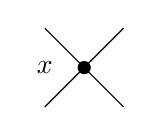
\begin{tikzpicture}[baseline=-0.1cm]
				\begin{feynhand}
					\vertex [dot] (x) at (0,0) {};
					\vertex [particle] (a) at (0.5,0.5);
					\vertex [particle] (b) at (-0.5,0.5);
					\vertex [particle] (c) at (0.5,-0.5);
					\vertex [particle] (d) at (-0.5,-0.5);
					\propag [] (a) to [] (x);
					\propag [] (b) to [] (x);
					\propag [] (c) to [] (x);
					\propag [] (d) to [] (x);
					\node at (-0.5,0) {$x$};
				\end{feynhand}
			\end{tikzpicture} \quad \sim \quad \frac{\lambda}{\mathrm{i}} \int \dd[4]{x};
		\]
		\item For each contraction we draw a line that connects a pair of vertices \[
			\begin{tikzpicture}[baseline=(a.base)]
				\begin{feynhand}
					\vertex (a) at (-1,0) {$x_1$};
					\vertex (b) at (1,0) {$x_2$};
					\propag [] (a) to [] (b);
				\end{feynhand}
			\end{tikzpicture} \quad \sim \quad \Delta_\text{F}(x_1 - x_2).
		\]
	\end{itemize}

	Hence, we can represent 
	\[
		\mathcal{M}(x_1, x_2) \quad  \supset \quad 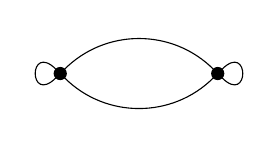
\begin{tikzpicture}[baseline = -0.1cm]
			\begin{feynhand}
				\vertex [particle] (hi) at (0,0);
				\vertex [dot] (a) at (-1,0) {};
				\vertex [dot] (b) at (1,0) {};
				\propag [] (a) to [in = 135, out = 225, loop] (a);
				\propag [] (b) to [in = 45, out = 315, loop] (b);
				\propag [] (a) to [out=45, in=135] (b);
				\propag [] (a) to [out=315, in=225] (b);
			\end{feynhand}
		\end{tikzpicture}.
	\]
	
	\subsubsection{Scattering in Scalar-Yukawa Theory}
	
	Recall, the Lagrangian is 
	\[
		\mathcal{L} = \partial_\mu \psi^* \partial^\mu \psi - M^2 \psi^* \psi + \frac{1}{2} \partial_\mu \phi \partial^\mu \phi - \frac{1}{2} m^2 \phi^2 - g \phi \psi^* \psi.
	\]
	
	The interaction picture field operators are
	\begin{align*}
		\hat \phi(x) &= \int \ddk{\vb p}{3} \frac{1}{\sqrt{2 E _{\vb p}}} \left[ \hat a _{\vb p} e ^{- \mathrm{i} p \cdot x} + \hat a^{\dagger}_{\vb p} e ^{+ \mathrm{i} p \cdot x} \right]\\
		\hat \psi(x) &= \int \ddk{\vb p}{3} \frac{1}{\sqrt{2 E _{\vb p}}} \left[ \hat b _{\vb p} e ^{- \mathrm{i} p \cdot x} + \hat c^{\dagger}_{\vb p} e ^{+ \mathrm{i} p \cdot x} \right]\\
		\hat \psi^{\dagger}(x) &= \int \ddk{\vb p}{3} \frac{1}{\sqrt{2 E _{\vb p}}} \left[ \hat b^{\dagger} _{\vb p} e ^{+ \mathrm{i} p \cdot x} + \hat c_{\vb p} e ^{- \mathrm{i} p \cdot x} \right]
	\end{align*}
	with
	\begin{align*}
		\hat a^{\dagger} \quad &\text{creates} \quad \text{$\phi$-particle},\\
		\hat b^{\dagger} \quad &\text{creates} \quad \text{$\psi$-particle},\\
		\hat c^{\dagger} \quad &\text{creates} \quad \text{$\bar \psi$-particle}.
	\end{align*}
	
	Consider a scattering process
	\[
		\psi + \psi \to \psi + \psi.
	\]

	This process can be seen as \needfig{$\psi \psi$-scattering}.

	The initial and final states are
	\[
		\ket{i} = \sqrt{2 E _{\vb p_1}} \sqrt{2 E _{\vb p_2}} \hat b^{\dagger}_{\vb p_1} \hat b^{\dagger}_{\vb p_2} \ket{0} \quad \text{and} \quad \ket{f} = \sqrt{2 E _{\vb p'_1}} \sqrt{2 E _{\vb p'_2}} \hat b^{\dagger} _{\vb p'_1} \hat b^{\dagger}_{\vb p'_2} \ket{0}.
	\]
	
	The scattering amplitude is
	\[
		\mathcal{A}_{i \to f} = \mel{f}{\hat S}{i}
	\]
	with
	\[
		\hat S = \mathcal{T}\left[ \exp(\frac{g}{\mathrm{i}}\int \dd[4]{x} \hat \phi \hat \psi^{\dagger}\hat \psi) \right].
	\]
	
	To get a non-zero answer, we need to bring down the exponential to terms like $\hat b \hat b \hat b^{\dagger} \hat b^{\dagger}$, which implies that the leading contribution occurs at $\mathcal{O}(g^2)$ order as 
	\[
		\mathcal{A}_{i \to f}^{(2)} := \frac{1}{2} \left( \frac{g}{\mathrm{i}} \right)^2 \int \dd[4]{x_1} \int \dd[4]{x_2} \mathcal{M}(x_1,x_2)
	\]
	with
	\begin{align*}
		\mathcal{M}(x_1,x_2) & = \mel{f}{\mathcal{T}[\hat \phi(x_1) \hat \psi^{\dagger}(x_1) \hat \psi(x_1)\hat \phi(x_2) \hat \psi^{\dagger}(x_2) \hat \psi(x_2)]}{i}\\
		& = \Delta_\text{F}^{(\phi)}(x_1 - x_2) \mel{f}{\nord{\hat \psi^{\dagger}(x_1)\hat \psi(x_1)\hat \psi^{\dagger}(x_2)\hat \psi(x_2)}}{i}\\
		& = \Delta_\text{F}^{(\phi)}(x_1 - x_2) \mel{f}{\hat \psi^{\dagger}(x_1) \hat \psi^{\dagger}(x_2) \hat \psi(x_1)\hat \psi(x_2)}{i}
	\end{align*}
	by applying Wick's theorem and only focusing on the non-zero term.

	An important aside: note that there is a very straightforward extension of contraction to $\hat \psi, \hat \psi^{\dagger}$ operators: \lec{15}
	\[
		\wick{\c{\hat \psi}(x_1)\c{\hat \psi}^{\dagger}(x_2)}:= \mel{0}{\mathcal{T}[\hat \psi(x_1)\hat \psi^{\dagger}(x_2)]}{0} = \int \ddk{p}{4} \frac{\mathrm{i} e ^{\mathrm{i} p \cdot (x_1 - x_2)}}{p^2 - M^2 + \mathrm{i} \epsilon} = \Delta_\text{F}^{(\psi)}(x_1 - x_2)
	\]
	and it is easy to find the contractions below vanishes:
	\[
		\wick{\c{\hat \psi}(x_1)\c{\hat \psi}(x_2)} = \wick{\c{\hat \psi^{\dagger}}(x_1) \c{\hat \psi}^{\dagger}(x_2)} = 0.
	\]

	Now we carry on to evaluate
	\begin{align*}
		\mathcal{N} & = \mel{f}{\hat \psi^{\dagger}(x_1)\hat \psi^{\dagger}(x_2) \hat \psi(x_1) \hat \psi(x_2)}{i}\\
		& = \mel{f}{\hat \psi^{\dagger}(x_1)\hat \psi^{\dagger}(x_2) \1 \hat \psi(x_1) \hat \psi(x_2)}{i}
	\end{align*}
	by inserting a complete set of states
	\[
		\1 = \sum _{\Psi} \dyad{\Psi}{\Psi}.
	\]

	We will find that only the vacuum state contributes among $\ket{\Psi}$'s , so
	\[
		\mathcal{N} = \mathcal{N}_i \mathcal{N}_f
	\]
	with
	\begin{align*}
		\mathcal{N}_i & = \mel{0}{\hat \psi(x_1)\hat \psi(x_2)}{i}\\
		& = \sqrt{2 E _{\vb p_1}} \sqrt{2 E _{\vb p_2}} \int \ddk{\vb p}{3} \int \ddk{\vb q}{3} \frac{1}{2 \sqrt{E _{\vb p} E _{\vb q}}} e ^{-\mathrm{i} p \cdot x_1 - \mathrm{i} q \cdot x_2} \underbrace{\mel{0}{\hat b _{\vb p} \hat b _{\vb q} \hat b^{\dagger}_{\vb p_1}\hat b^{\dagger}_{\vb p_2}}{0}}_{\text{(A)}}.
	\end{align*}

	Evaluate (A) using
	\[
		[\hat b_{\vb p}, \hat b^{\dagger}_{\vb p'}] = (2 \pi)^3 \delta^{(3)} (\vb p - \vb p')
	\]
	to get
	\[
		\text{(A)} = (2 \pi)^6 \left( \delta ^{(3)}(\vb p_1 - \vb p) \delta ^{(3)}(\vb p_2 - \vb q) + \delta ^{(3)}(\vb p_2 - \vb p) \delta ^{(3)}(\vb p_1 - \vb q)\right).
	\]
	
	Now go back and do the $\vb p$ and $\vb q$ integrals, we have
	\[
		\mathcal{N}_i = \mel{0}{\hat \psi(x_1) \hat \psi(x_2)}{i} = \left( e ^{-\mathrm{i} p_1 \cdot x_1 - \mathrm{i} p_2 \cdot x_2} + e ^{- \mathrm{i} p_2 \cdot x_1 - \mathrm{i} p_1 \cdot x_2} \right)
	\]
	and a similar calculation for 
	\[
		\mathcal{N}_f = \mel{f}{\hat \psi^{\dagger}(x_1)\hat \psi^{\dagger}(x_2)}{0} = \left( e ^{+\mathrm{i} p'_1 \cdot x_1 + \mathrm{i} p'_2 \cdot x_2} + e ^{+ \mathrm{i} p'_2 \cdot x_1 + \mathrm{i} p'_1 \cdot x_2} \right).
	\]

	Thus
	\begin{align*}
		\mathcal{A}^{(2)}_{i \to f} & = \frac{1}{2} \left( \frac{g}{\mathrm{i}} \right)^2 \int \dd[4]{x_1} \int \dd[4]{x_2} \mathcal{N}_f \mathcal{N}_i \int \ddk{k}{4} \frac{\mathrm{i} e ^{\mathrm{i} k \cdot (x_1 - x_2)}}{k^2 - m^2 + \mathrm{i} \epsilon}\\
		& = \frac{1}{2} \left( \frac{g}{\mathrm{i}} \right)^2 \int \ddk{k}{4} \frac{\mathrm{i}}{k_2 - m_2 + \mathrm{i} \epsilon} \int \dd[4]{x_1} \int \dd[4]{x_2} \times\\
		& \qquad \times \left[ e ^{\mathrm{i}x_1 \cdot(k + p'_1 - p_1)} e ^{\mathrm{i}x_2 \cdot (k - p'_2 + p_2)} + e ^{\mathrm{i} x_1 \cdot(k + p'_2 - p_1)} e ^{\mathrm{i} x_2 \cdot (k - p'_1 + p_2)} + (x_1 \leftrightarrow x_2)\right].
	\end{align*}
	
	Now do the $x_1, x_2$ integrals,
	\[
		\int \dd[4]{x} e ^{\mathrm{i} p \cdot x} = (2 \pi)^4 \delta ^{(4)}(p)
	\]
	and do the $k$ integrals which saturate one $\delta$-function, we finally have
	\[
		\mathcal{A}^{(2)}_{i \to f} = \mathrm{i} (- \mathrm{i} g)^2 (2 \pi)^4 \delta ^{(4)}(p_1 + p_2 - p'_1 - p'_2) \left[ \frac{1}{(p_1 - p'_1)^2 - m^2 + \mathrm{i} \epsilon} + \frac{1}{(p_1 - p'_2)^2 - m^2 + \mathrm{i} \epsilon} \right].
	\]

	A few properties of $\mathcal{A}^{(2)}_{i \to f}$:
	\begin{itemize}
		\item $\delta ^{(4)}$ imposes conservation of energy and momentum \[
			p'_1 + p'_2 = p_1 + p_2.
		\]
		\item We can check $(p_1 - p'_1)^2, (p_1 - p'_2)^2 < 0$ so we can erase the $\mathrm{i} \epsilon$-prescription if needed. 
	\end{itemize}
	
	\subsection{Feynman Diagrams}
	
	Contributions to 
	\[
		\mel{f}{\hat S - 1}{i}
	\]
	is in one-to-one correspondence to certain \emph{Feynman diagrams}.

	\begin{itemize}
		\item We first choose a direction of time;
		\item Draw external line for each particle in $\ket{i}$ and $\ket{f}$; \[
			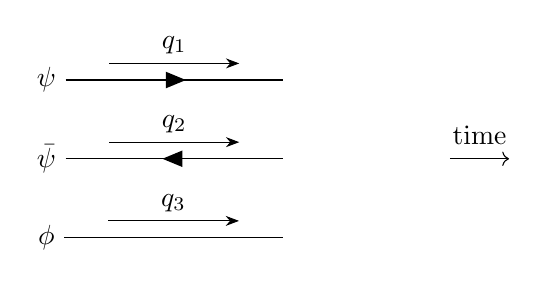
\begin{tikzpicture}
				\begin{feynhand}
					\vertex (p) at (0,1) {$\psi$};
					\vertex [particle] (pn) at (3,1);
					\vertex (ap) at (0,0) {$\bar \psi$};
					\vertex [particle] (apn) at (3,0);
					\vertex (f) at (0,-1) {$\phi$};
					\vertex [particle] (fn) at (3,-1);
					\propag [fer, mom={$q_1$}] (p) to [] (pn);
					\propag [antfer, mom={$q_2$}] (ap) to [] (apn);
					\propag [mom={$q_3$}] (f) to [] (fn);
					\node (t1) at (5,0);
					\node (t2) at (6,0);
					\draw [->] (t1) to (t2);
					\node (t) at (5.5,0.3) {time};
				\end{feynhand}
			\end{tikzpicture}
		\]
		\item Connect the external lines together with \emph{vertices} \[
			\begin{tikzpicture}
				\begin{feynhand}
					\vertex [particle] (m) at (0,0);
					\vertex (i) at (-2.121,0) {};
					\vertex (f1) at (1.5,1.5) {};
					\vertex (f2) at (1.5,-1.5) {};
					\propag [] (i) to [] (m);
					\propag [fer] (m) to [] (f1);
					\propag [antfer] (m) to [] (f2);
				\end{feynhand}
			\end{tikzpicture}
		\]
		\item Draw internal lines connecting vertices.
	\end{itemize}

	Now, for $\psi \psi \to \psi \psi$ scattering, the leading order diagrams are (where the time flows in \emph{vertical} direction)
	\[
		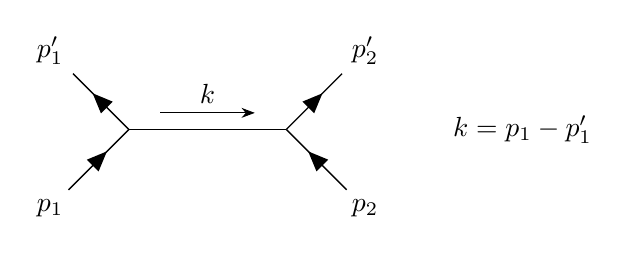
\begin{tikzpicture}
			\begin{feynhand}
				\vertex (i1) at (-1,-1) {$p_1$};
				\vertex (i2) at (3,-1) {$p_2$};
				\vertex (f1) at (-1,1) {$p'_1$};
				\vertex (f2) at (3,1) {$p'_2$};
				\vertex [particle] (a) at (0,0);
				\vertex [particle] (b) at (2,0);
				\propag [fer] (i1) to [] (a);
				\propag [fer] (a) to [] (f1);
				\propag [fer] (i2) to [] (b);
				\propag [fer] (b) to [] (f2);
				\propag [mom={$k$}] (a) to [] (b);
				\node (c) at (5,0) {$k = p_1 - p'_1$};
			\end{feynhand}
		\end{tikzpicture}
	\]
	and
	\[
		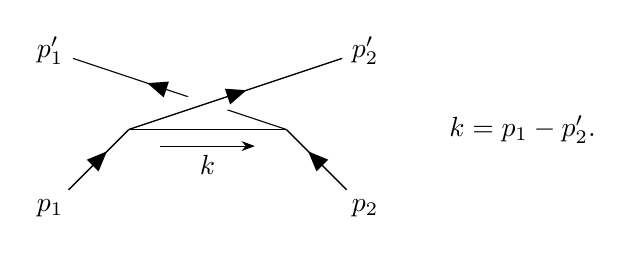
\begin{tikzpicture}
			\begin{feynhand}
				\vertex (i1) at (-1,-1) {$p_1$};
				\vertex (i2) at (3,-1) {$p_2$};
				\vertex (f1) at (-1,1) {$p'_1$};
				\vertex (f2) at (3,1) {$p'_2$};
				\vertex [particle] (a) at (0,0);
				\vertex [particle] (b) at (2,0);
				\propag [fer] (i1) to [] (a);
				\propag [with arrow=0.6] (b) to [] (f1);
				\propag [fer, top] (a) to [] (f2);
				\propag [fer] (i2) to [] (b);
				\propag [mom'={$k$}] (a) to [] (b);
				\node (c) at (5,0) {$k = p_1 - p'_2$.};
			\end{feynhand}
		\end{tikzpicture}
	\]
	
	\subsubsection{Feynman Rules}
	To translate the diagrams to mathematical expressions, we have the \emph{Feynman rules}.
	\begin{itemize}
		\item Assign propagators to each internal line \[
			\begin{tikzpicture}
				\begin{feynhand}
					\vertex (p) at (0,0.5) {};
					\vertex [particle] (pn) at (3,0.5);
					\vertex (ap) at (0,0) {};
					\vertex [particle] (apn) at (3,0);
					\vertex (f) at (0,-1.5) {};
					\vertex [particle] (fn) at (3,-1.5);
					\propag [fer, mom={$k$}] (p) to [] (pn);
					\propag [antfer, mom'={$k$}] (ap) to [] (apn);
					\propag [mom={$k'$}] (f) to [] (fn);
					\node (t) at (5.5,0.25) {$\sim \quad \dfrac{\mathrm{i}}{k^2 - M^2 + \mathrm{i} \epsilon}$ };
					\node (t) at (5.5,-1.5) {$\sim \quad \dfrac{\mathrm{i}}{k'^2 - m^2 + \mathrm{i} \epsilon}$ };
				\end{feynhand}
			\end{tikzpicture}
		\]
		\item Each vertex gives \[
			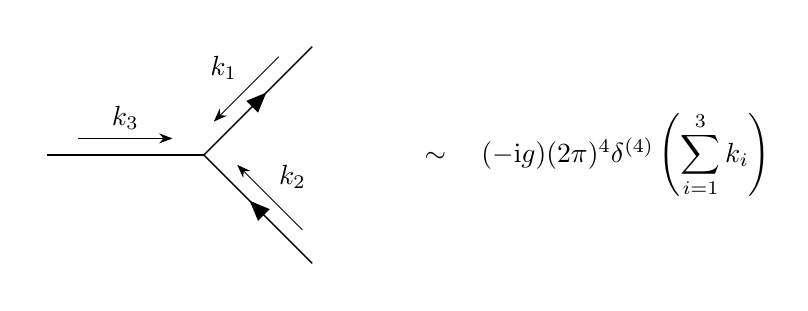
\begin{tikzpicture}
				\begin{feynhand}
					\vertex [particle] (m) at (0,0);
					\vertex (i) at (-2.121,0) {};
					\vertex (f1) at (1.5,1.5) {};
					\vertex (f2) at (1.5,-1.5) {};
					\propag [mom = {$k_3$}] (i) to [] (m);
					\propag [fer, revmom={$k_1$}] (m) to [] (f1);
					\propag [antfer,revmom={$k_2$}] (m) to [] (f2);
					\node (c) at (5,0) {$\sim \quad (-\mathrm{i} g) (2 \pi)^4 \delta ^{(4)}\left( \displaystyle\sum _{i = 1}^3 k_i\right)$};
				\end{feynhand} 
			\end{tikzpicture}
		\]
		\item Integrate over internal momenta.
	\end{itemize}
	\newpage
	\section{Fermions}
	So far, we considered scalar fields,
	\[
		\phi(x) \xrightarrow{\text{L.T.}} \phi(\Lambda^{-1} \cdot x)
	\]
	under $x^\mu \to x'^\mu = \LT{\mu}{\nu} x ^{\nu}$.

	$\hat \phi$ creates particles with \emph{spin zero}. For a massive particle, the \emph{spin} is the the angular momentum in the rest frame, 
	\[
		\mel{\vb 0}{\hat{\vb J}}{\vb 0} = 0.
	\]
	
	The non-relativistic description of spin uses 
	\[
		\hat{\vb S} = (\hat S_x, \hat S_y, \hat S_z), \quad \hat S^2, \quad \hat S_z
	\]
	and particles are of spin $s = 0, \frac{1}{2}, 1, \frac{3}{2}, \cdots$ has $(2s+1)$-spin states with
	\[
		-s \leq s_z \leq s,
	\]
	labelled by $\ket{s,s_z}$ satisfying
	\[
		\hat S^2 \ket{s,s_z} = s(s+1) \ket{s,s_z} \quad \text{and} \quad \hat S_z \ket{s,s_z} = s_z \ket{s,s_z}.
	\]
	
	Electrons have spin $\frac{1}{2}$, i.e.\ each has two states $\ket{\uparrow}, \ket{\downarrow}$. Now we need a relativistic way to describe such spin.

	\subsection{Relativistic Spin}
	We need fields which transform in non-trivial representations of Lorentz group. \lec{16}

	The Lorentz group is
	\[
		G_L = \{\Lambda \in \Mat_4(\mathbb{R}) : \Lambda \eta \Lambda^T = \eta, \det \Lambda = +1\} = \SO(3,1).
	\]
	
	\begin{defi}
		A \emph{representation $D$ of $G_L$ of dimension $N$} is a smooth map 
	\[
		D : G_L \to \Mat_N(\mathbb{C})
	\]
	which is also a group homomorphism, i.e.\ 
	\[
		D[\Lambda_1] \cdot D[\Lambda_2] = D[\Lambda_1 \cdot \Lambda_2] \quad \forall \Lambda_1, \Lambda_2 \in G_L.
	\]

	The matrices $D[\Lambda]$ act on vectors in some \emph{representation space} $\mathcal{V} \simeq \mathbb{C}^N$.
	\end{defi}

	We can explicitly write $D[\Lambda]_{AB}$ for $A,B = 1, \cdots, N$.
	
	\begin{defi}
		A field $\Psi : \mathbb{R} ^{3,1} \to \mathbb{C}^N$ \emph{transforms in the representation $D$ of $G_L$} if, under $x^\mu \to \LT{\mu}{\nu} x^\nu$ we have
		\[
			\Psi_A(x) \to \Psi'_A(x) := \sum _{B = 1}^N D[\Lambda]_{AB} \Psi_B(\Lambda^{-1} \cdot x).
		\]
	\end{defi}

	\begin{ex}
		\ 
		\begin{itemize}
			\item Scalar field $\phi(x) \to \phi(\Lambda^{-1} \cdot x)$ has $N = 1$, with \emph{trivial representation} $D[\Lambda] = 1, \forall \Lambda \in G_L$;
			\item 4-vector field $A^\mu (x) \to \LT{\mu}{\nu} A ^\nu(\Lambda^{-1} \cdot x)$ has $N = 4$, with \emph{fundamental representation} $D[\Lambda] = \Lambda$. 
		\end{itemize}
	\end{ex}

	We want to construct new representations of $G_L$. We work with the \emph{Lie algebra} $\mathbb{L}(G_L)$ for convenience. We will use the \emph{exponential map}
	\[
		\Exp : \mathbb{L}(G_L) \to G_L
	\]
	which is bijective in some neighbourhood of identity element.

	\begin{defi}
		A \emph{representation of Lie algebra $\mathbb{L}(G_L)$} with dimension $N$ is a linear map 
		\[
			R : \mathbb{L}(G_L) \to \Mat_N(\mathbb{C})
		\]
		which preserves the Lie bracket, i.e.\ $\forall X,Y \in \mathbb{L}(G_L)$ 
		\[
			R([X,Y]) = [R(X), R(Y)].
		\]
	\end{defi}
	
	Given a representation $R$ of $\mathbb{L}(G_L)$, we can define
	\[
		D[\Lambda] = \exp(R(X)) \quad \text{for} \quad \Lambda = \Exp(X).
	\]
	$D$ yields a representation of the \emph{universal cover} $\tilde G_L = \text{Spin}(3,1) \simeq \SL(2, \mathbb{C})$ of Lorentz group $G_L = \SO(3,1)$. In this case, the covering group $\SL(2,\mathbb{C})$ is not isomorphic to $\SO(3,1)$ but a double cover of it, i.e.\ there exists a global 2:1 map
	\[
		e : \tilde G_L \xrightarrow{2:1} G_L.
	\]
	(Or we can say, $\SO(3,1) \simeq \SL(2,\mathbb{C})/\mathbb{Z}_2$.)

	For the case of rotations in $\mathbb{R}^3$, 
	\[
		G = \SO(3) \quad \text{with cover} \quad \tilde G = \SU(2)
	\]
	with a map
	\[
		e : \SU(2) \xrightarrow{2:1} \SO(3).
	\]
	(Again, we can say $\SO(3) \simeq \SU(2)/\mathbb{Z}_2$.)

	Here we consider \emph{proper Lorentz transformations}, $G_L = \SO(3,1)$ with
	\[
		\Lambda = \Exp(\omega)
	\]
	and in components 
	\[
		\LT{\mu}{\nu} = \delta^\mu_\nu + \omega\indices{^\mu_\nu} + \frac{1}{2} \omega\indices{^\mu_\rho} \omega\indices{^\rho_\nu} + \cdots 
	\]
	
	The condition of $\Lambda \in G_L$ is $\Lambda \eta \Lambda^T = \eta$, so we require 
	\[
		\omega ^{\mu \nu} + \omega ^{\nu \mu} = 0.
	\]
	Thus the Lie algebra is
	\[
		\mathbb{L}(G_L) = \{\omega \in \Mat_4(\mathbb{R}) : \omega + \omega^T = 0\}.
	\]

	Hence, the number of generators is 
	\[
		\frac{1}{2} (4 \times 3) = 6 \quad \sim \quad \text{3 rotations} + \text{3 boosts}.
	\]
	
	The natural basis consists of 
	\[
		(M ^{\rho \sigma})^{\mu \nu} = \eta ^{\rho \mu} \eta ^{\sigma \nu} - \eta ^{\sigma \mu} \eta ^{\rho \nu}.
	\]

	Note that the indices $\rho,\sigma$ labels different generators, while $\mu,\nu$ gives the entries in the representation matrices.

	For example
	\[
		(M ^{01})^{\mu \nu} = \mqty(0 & 1 & 0 & 0\\ -1 & 0 & 0 & 0\\ 0 & 0 & 0 & 0\\ 0 & 0 & 0 & 0)
	\]
	which is the generator of boost along $x$-axis.

	A general element of $\mathbb{L}(G_L)$ is 
	\[
		\omega\indices{^\mu_\nu} = \frac{1}{2} \Omega _{\rho \sigma} \left( M ^{\rho \sigma} \right)\indices{^\mu_\nu}
	\]
	where we take $\Omega _{\rho \sigma} = - \Omega _{\sigma \rho}$ to be the parameters of a general Lie algebra element.

	The resulting Lie bracket should be 
	\begin{equation}
		[M ^{\rho \sigma}, M ^{\tau \nu}] = \eta ^{\sigma \tau} M ^{\rho \nu} - \eta ^{\rho \tau} M ^{\sigma \nu} + \eta ^{\rho \nu} M ^{\sigma \tau} - \eta ^{\sigma \nu} M ^{\rho \tau}.
		\label{eq:4.1.1}
	\end{equation}

	The Lie group elements $\Lambda \in G_L$ are then
	\[
		\Lambda = \Exp\left( \frac{1}{2} \Omega _{\rho \sigma} M ^{\rho \sigma} \right).
	\]
	
	Now we turn to something else.

	\begin{defi}
		The \emph{Clifford algebra} with elements $\gamma^0, \gamma^1, \gamma^2, \gamma^3$ are such that the \emph{anticommutators} obey 
	\begin{equation}
		\{\gamma^\mu, \gamma^\nu\} := \gamma^\mu \gamma^\nu + \gamma^\nu \gamma^\mu = 2 \eta ^{\mu \nu} \1_4.
		\label{eq:4.1.2}
	\end{equation}
	\end{defi}

	We want to find representations of Clifford algebra.

	Introducing the Pauli matrices
	\[
		\bm \sigma = \left( \mqty(\pmat{1}),\mqty(\pmat{2}),\mqty(\pmat{3}) \right)
	\]
	which obeys (for $i,j = 1,2,3$)
	\[
		\{\sigma^i , \sigma^j\} = 2 \delta ^{ij} \1_2.
	\]
	
	\begin{defi}
		The \emph{simple representation} (unique irrep of Clifford algebra up to conjugation $\gamma^\mu \to V \gamma^\mu V^{-1}$) is 
	\begin{equation}
		\gamma^0 = \mqty(0 & \1_2\\ \1_2 & 0), \quad \gamma^i = \mqty(0 & \sigma^i\\ -\sigma^i & 0).
		\label{eq:4.1.3}
	\end{equation}
	This is also called the \emph{Weyl representation}.
	\end{defi}

	Now, define 
	\begin{equation}
		S ^{\rho \sigma} := \frac{1}{4} [\gamma^\rho, \gamma^\sigma] = \frac{1}{2} \gamma^\rho \gamma^\sigma - \frac{1}{4} \{\gamma^\rho, \gamma^\sigma\} = \frac{1}{2} \gamma^\rho \gamma^\sigma - \frac{1}{2} \eta ^{\rho \sigma}
		\label{eq:4.1.4}
	\end{equation}
	and check Question 3, Sheet 3, we find
	\begin{equation}
		[S ^{\mu \nu}, S ^{\rho \sigma}] = \eta ^{\nu \rho} S ^{\mu \sigma} - \eta ^{\mu \rho} S ^{\nu \sigma} + \eta ^{\mu \sigma} S ^{\nu \rho} - \eta ^{\nu \sigma} S ^{\mu \rho}.
		\label{eq:4.1.5}
	\end{equation}

	$S ^{\mu \nu}$ provide a 4d representation of $\mathbb{L}(G_L)$. Exponentiate to give a representation of universal cover $\tilde G_L = \text{Spin}(3,1) \xrightarrow{2:1} G_L = \SO(3,1)$. For 
	\[
		\Lambda = \Exp \left( \frac{1}{2} \Omega _{\rho \sigma} M ^{\rho \sigma} \right)
	\]
	the new representation is
	\[
		S[\Lambda] = \Exp \left( \frac{1}{2} \Omega _{\rho \sigma} S ^{\rho \sigma} \right).
	\]
	 
	It is a new four-dimensional representation 
	\[
		S : \tilde G_L \to \Mat_4 (\mathbb{C})
	\]
	but not well-defined as $G_L \to \Mat_4(\mathbb{C})$. We call this representation a \emph{spinor representation}.
	
	\lec{17}

	We will focus on rotations by setting parameters $\Omega$ to be
	\[
		\Omega _{ij} = - \epsilon _{ijk} \varphi^k
	\]
	and denote $\bm \varphi = (\varphi^1, \varphi^2, \varphi^3)$.

	The generators are
	\begin{align*}
		S ^{ij} & = \frac{1}{4} [\gamma^i, \gamma^j] \overset{i \neq j}{=} \frac{1}{2} \gamma^i \gamma^j\overset{\text{chiral}}{=} \frac{1}{2} \mqty(0 & \sigma^i\\ - \sigma^i & 0) \mqty(0 & \sigma^j \\ - \sigma^j & 0)\\
		& = \frac{1}{2} \mqty(- \sigma^i \sigma^j & 0 \\ 0 & - \sigma^i \sigma^j) = - \frac{\mathrm{i}}{2} \epsilon ^{ijk} \mqty(\sigma^k & 0 \\ 0 & \sigma^k).
	\end{align*}

	Then we can evaluate in this case
	\[
		S[\Lambda] = \Exp\left( \frac{1}{2} \Omega _{ij} S ^{ij} \right) = \mqty( e ^{+ \mathrm{i} \bm \varphi \vdot \bm \sigma/2} & 0 \\ 0 & e ^{+\mathrm{i} \bm \varphi \vdot \bm \sigma/2}).
	\]
	
	Specialising further by setting $\varphi^1 = \varphi^2 = 0$, we get
	\[
		S[\varphi^3] = S[\Lambda]\big| _{\varphi^1 = \varphi^2 = 0} = \mqty(\dmat{e ^{+\mathrm{i} \varphi^3/2},e ^{-\mathrm{i} \varphi^3/2},e ^{+\mathrm{i} \varphi^3/2},e ^{-\mathrm{i} \varphi^3/2}}).
	\]

	The corresponding Lorentz group element is
	\[
		\Lambda = \Exp \left( \frac{1}{2} \Omega _{ij} M ^{ij} \right) \quad \text{with} \quad \Omega _{ij} = - \epsilon _{ijk} \varphi^k
	\]
	and setting $\varphi^1, \varphi^2 = 0$.

	Then
	\[
		\Lambda[\varphi^3] = \Exp \left( - \varphi^3 M ^{12} \right)
	\]
	and recall
	\[
		M ^{12} = \mqty(0 & 0 & 0 & 0\\ 0 & 0 & -1 & 0 \\ 0 & 1 & 0 & 0\\ 0 & 0 & 0 & 0) 
	\]
	we get
	\[
		\Lambda[\varphi^3] = \mqty(1 & 0 & 0 & 0 \\ 0 & \cos \varphi^3 & \sin \varphi^3 & 0 \\ 0 & -\sin \varphi^3 & \cos \varphi^3 & 0 \\ 0 & 0 & 0 & 1).
	\]
	
	If we set $\varphi^3 = 2 \pi$ we find
	\[
		\Lambda [ \varphi^3 = 2 \pi] = \1_4 \quad \text{but} \quad S[\varphi^3 = 2 \pi] = - \1_4.
	\]
	
	This suggests that the spinor representation is actually a representation of the \emph{double cover} of the Lorentz group but the group itself.

	\subsection{Spinor Representation}

	Recall the Clifford algebra $\gamma^\mu$ with $\mu = 0,1,2,3$. The key property is that, if we conjugate $\gamma^\mu$ with the spinor representation matrices, we get
	\begin{equation}
		S[\Lambda]^{-1} \gamma^\mu S[\Lambda] = \LT{\mu}{\nu} \gamma^\nu.
		\label{eq:4.2.1}
	\end{equation}  

	Check at infinitesimal level and recall
	\[
		\Lambda = \Exp \left( \frac{1}{2} \Omega _{\rho \sigma} \mathcal{M}^{\rho \sigma} \right)
	\]
	the RHS of (\ref{eq:4.2.1}) is 
	\begin{align*}
		\text{RHS} &\approx \gamma^\mu + \frac{1}{2} \Omega _{\rho \sigma} (\mathcal{M}^{\rho \sigma})\indices{^\mu _\nu} \gamma^\nu + \mathcal{O}(\Omega^2)\\
		& = \gamma^\mu + \frac{1}{2} \Omega _{\rho \sigma} \left( \eta ^{\rho \mu} \gamma^\sigma - \eta ^{\sigma \mu} \gamma^\rho \right) + \mathcal{O}(\Omega^2)
	\end{align*}
	by using $(\mathcal{M}^{\rho \sigma})\indices{^\mu_\nu} = \eta ^{\rho \mu}\delta^\sigma_\nu - \eta ^{\sigma \mu} \delta^\rho_\nu$. For the LHS, recall 
	\[
		S[\Lambda] = \Exp \left( \frac{1}{2} \Omega _{\rho \sigma} S ^{\rho \sigma} \right)
	\]
	and we get 
	\begin{align*}
		\text{LHS} & \approx \left( \1_4 - \frac{1}{2} \Omega _{\rho \sigma} S ^{\rho \sigma} \right) \gamma^\mu \left( \1_4 + \frac{1}{2} \Omega _{\rho \sigma} S ^{\rho \sigma} \right) + \mathcal{O}(\Omega^2)\\
		& \approx \gamma^\mu + \frac{1}{2} \Omega _{\rho \sigma} [\gamma^\mu, S ^{\rho \sigma}] + \mathcal{O}(\Omega^2).
	\end{align*}
	
	At linear order, (\ref{eq:4.2.1}) is equivalent to 
	\begin{equation}
		[\gamma^\mu , S ^{\rho \sigma}] = \eta ^{\rho \mu} \gamma^\sigma - \eta ^{\sigma \mu} \gamma^\rho.
		\label{eq:4.2.2}
	\end{equation}

	\begin{exer}
		Prove that (\ref{eq:4.2.2}) holds.
	\end{exer}

	\subsection{Spinor Fields}

	\begin{defi}
		A \emph{spinor field} is a map 
		\[
			\psi : \mathbb{R} ^{3,1} \to \mathbb{C}^4, \quad x \mapsto \psi^\alpha (x) \in \mathbb{C} \quad \text{with} \quad \alpha = 1,2,3,4.
		\]
		where $\alpha$ are the \emph{spinor index}. It has transformation property under Lorentz transformations $\Lambda \in G_L$, $x^\mu \to \LT{\mu}{\nu}x^\nu$, 
		\begin{equation}
			\psi^\alpha (x) \to \psi'^\alpha (x) := S[\Lambda]\indices{^\alpha_\beta} \psi^\beta(\Lambda^{-1} \cdot x)
			\label{eq:4.3.1}
		\end{equation}
		where summation convention is assumed. 
	\end{defi}

	Usually the indices can be suppressed, and one can write compactly
		\[
			\psi(x) \to S[\Lambda] \cdot \psi(\Lambda^{-1} \cdot x).
		\]

	The key property is that, under $2 \pi$ rotation, 
	\[
		\psi(x) \to - \psi(x).
	\]
	
	Now we want to construct Lagrangian out of such spinor fields. 

	First, consider the spacetime derivative $\partial_\mu \psi(x)$, it has transformation property (c.f.\ the scalar case)
	\[
		\partial_\mu \psi(x) \to (\Lambda^{-1})\indices{^\nu_\mu} S[\Lambda]\cdot \partial_\nu \psi(\Lambda^{-1} \cdot x).
	\]
	 
	Secondly, look at the conjugate field $\psi^{\dagger}_\alpha(x)$, its transformation property is
	\begin{equation}
		\psi^{\dagger}(x) \to \psi^{\dagger} \cdot S[\Lambda]^{\dagger}.
		\label{eq:4.3.2}
	\end{equation}
	An important point to note here is: the representation $S$ is \emph{not unitary}, so in general $S[\Lambda]^{\dagger} \neq S[\Lambda]^{-1}$. 

	\begin{thm}
		A simple, non-compact Lie group has no non-trivial, finite-dimensional unitary representations.
	\end{thm}

	The simplest non-trivial representation of the Lorentz group is its fundamental representation $\Lambda \in \SO(3,1)$, which has the property $\Lambda \eta \Lambda^T = \eta$ not equivalent to $\Lambda \Lambda^T = \1_4.$
	
	We want to further investigate the conjugation. The Clifford algebra
	\[
		\{\gamma^\mu, \gamma^\nu\} = 2 \eta ^{\mu \nu} \1_4
	\]
	leads to 
	\[
		(\gamma^0)^2 = \1_4 \quad \text{and} \quad (\gamma^i)^2 = - \1_4
	\]
	so $\gamma^0$ has real eigenvalues and is Hermitian, and $\gamma^i$ have imaginary eigenvalues and are anti-Hermitian, i.e.\ 
	\[
		(\gamma^0)^{\dagger} = \gamma^0 \quad \text{and} \quad (\gamma^i)^{\dagger} = - \gamma^i.
	\]
	
	We can write
	\[
		\gamma^0 \gamma^0 \gamma^0 = \gamma^0 = (\gamma^0)^{\dagger}
		\tag{$\alpha$}
		\label{eq:4.alpha}
	\]
	and one finds
	\[
		\gamma^0 \gamma^i \gamma^0 = \gamma^0 \{\gamma^i, \gamma^0\} - \gamma^0 \gamma^0 \gamma^i = - \gamma^i = (\gamma^i)^{\dagger}.
		\tag{$\beta$}
		\label{eq:4.beta}
	\]
	
	Combining (\ref{eq:4.alpha}) and (\ref{eq:4.beta}) we conclude 
	\[
		(\gamma^\mu)^{\dagger} = \gamma^0 \gamma^\mu \gamma^0.
	\]
	
	Now we take the Hermitian conjugte of $S _{\mu \nu}$ \lec{18}
	\begin{align*}
		(S _{\mu \nu})^{\dagger} & = \frac{1}{4} \left( [\gamma^\mu, \gamma^\nu] \right)^{\dagger} = \frac{1}{4} \left( [{\gamma^\nu}^{\dagger}, {\gamma^\mu}^{\dagger}] \right)\\
		& = \frac{1}{4} [\gamma^0 \gamma^\nu \gamma^0, \gamma^0 \gamma^\mu \gamma^0] = \frac{1}{4} \gamma^0 [\gamma^\nu, \gamma^\mu]\gamma^0\\
		& = - \frac{1}{4} \gamma^0 [\gamma^\mu, \gamma^\nu] \gamma^0
	\end{align*}
	i.e.\ we have
	\[
		(S ^{\mu \nu})^{\dagger} = - \gamma^0 S ^{\mu \nu}\gamma^0.
	\]
	
	So
	\begin{align*}
		S[\Lambda]^{\dagger} & = \left[\Exp \left( \frac{1}{2} \Omega _{\rho \sigma} S ^{\rho \sigma} \right)\right]^{\dagger} = \Exp \left( \frac{1}{2} \Omega _{\rho \sigma} \left( S ^{\rho \sigma} \right)^{\dagger} \right) \\
		& = \Exp\left( - \frac{1}{2} \Omega _{\rho \sigma} \gamma^0 S ^{\rho \sigma} \gamma^0 \right)\\
		& = \gamma^0 \Exp \left( - \frac{1}{2} \Omega _{\rho \sigma} S ^{\rho \sigma} \right) \gamma^0
	\end{align*}
	thus
	\begin{equation}
		\left( S[\Lambda] \right)^{\dagger} = \gamma^0 S[\Lambda]^{-1} \gamma^0.
		\label{eq:4-11}
	\end{equation}

	This means $S[\Lambda]$ is not a unitary representation.

	Consider spinor field $\psi^\alpha(x)$, the Hermitian conjugate transforms as 
	\[
		\psi^{\dagger}(x) \to \psi^{\dagger}(\Lambda^{-1} \cdot x) S[\Lambda]^{\dagger} = \psi^{\dagger} (\Lambda^{-1} \cdot x) \gamma^0 S[\Lambda]^{-1} \gamma^0.
	\]

	So, $\psi^{\dagger} \psi$ is \emph{not} a Lorentz scalar. To proceed, we have the following definition.

	\begin{defi}
		The \emph{Dirac adjoint} of a spinor field $\psi(x)$ is a field 
		\[
			\bar \psi(x) : = \psi^{\dagger}(x) \gamma^0.
		\]
	\end{defi}	

	Under Lorentz transformation $\Lambda \in G_L$, we have
	\[
		\bar \psi(x) \to \bar \psi'(x) = \psi^{\dagger}(\Lambda^{-1} \cdot x) \gamma^0 S[\Lambda]^{-1} \gamma^0 \gamma^0 = \bar \psi(\Lambda^{-1} \cdot x) S[\Lambda]^{-1}.
	\]

	Now define, 
	\[
		\Sigma(x) = \bar \psi(x) \psi(x),
	\]
	under Lorentz transformation, it transforms as 
	\[
		\Sigma(x) \xrightarrow{\Lambda} \bar \psi(\Lambda^{-1} \cdot x) S[\Lambda]^{-1} S[\Lambda] \psi(\Lambda^{-1} \cdot x) = \bar \psi(\Lambda^{-1}\cdot x) \psi(\Lambda^{-1} \cdot x) = \Sigma(\Lambda^{-1} \cdot x)
	\]
	so we can conclude that $\Sigma(x)$ is a scalar field.

	\begin{clm}
		We can also form vector field
		\[
			V^\mu(x) = \bar \psi(x) \gamma^\mu \psi(x).
		\]
	\end{clm}
	\begin{proof}
		Under Lorentz transformation $\Lambda \in G_L$,
		\begin{align*}
			V^\mu(x) & \xrightarrow{\Lambda} \bar \psi(\Lambda^{-1} \cdot x) S[\Lambda]^{-1} \gamma^\mu S[\Lambda] \psi(\Lambda^{-1} \cdot x)\\
			& \overset{(\ref{eq:4.2.1})}{=} \LT{\mu}{\nu} \bar \psi(\Lambda^{-1} \cdot x) S[\Lambda]^{-1} \gamma^\nu S[\Lambda] \psi(\Lambda^{-1} \cdot x)\\
			&\ = \LT{\mu}{\nu} V^\nu (\Lambda^{-1} \cdot x).
		\end{align*}
	\end{proof}

	\subsection{Dirac Action}

	We want an action for the spinor field. We want it to be 
	\begin{itemize}
		\item Lorentz invariant,
		\item Real.
	\end{itemize}
	To achieve this, we work with Lagrangian density 
	\[
		S = \int \dd[4]{x} \mathcal{L}(x)
	\]
	where 
	\begin{itemize}
		\item $\mathcal{L}$ is a scalar field;
		\item $\mathcal{L}$ is real.	
	\end{itemize}
	
	Write down the \emph{Dirac Lagrangian}
	\[
		\mathcal{L}(x) = \mathcal{L}_1 + \mathcal{L}_2 = \bar \psi(x) \mathrm{i} \gamma^\mu \partial_\mu \psi(x) - m \bar \psi(x) \psi(x).
	\]
	
	\begin{clm}
		$\mathcal{L}(x)$ is a scalar.
	\end{clm}

	\begin{proof}
		We can already confirm $\mathcal{L}_2(x)$ is a scalar. It suffices to check $\mathcal{L}_1(x)$. Consider a Lorentz transformation $\Lambda \in G_L$, 
		\begin{align*}
			\mathcal{L}_1(x) & = \bar \psi(x) \mathrm{i} \gamma^\mu \partial_\mu \psi(x)\\
			& \xrightarrow{\Lambda} \bar \psi(\Lambda^{-1} \cdot x) S[\Lambda]^{-1} \mathrm{i} \gamma^\mu \left( \Lambda^{-1} \right)\indices{^\nu_\mu} S[\Lambda] \partial_\nu \psi(\Lambda^{-1} \cdot x)\\
			& = \mathrm{i} \bar \psi(\Lambda^{-1} \cdot x) \left( S[\Lambda]^{-1} \gamma^\mu S[\Lambda] \right) \left( \Lambda^{-1} \right)\indices{^\nu _\mu} \partial_\nu \psi(\Lambda^{-1} \cdot x)\\
			& \overset{(\ref{eq:4.2.1})}{=} \mathrm{i} \bar \psi(\Lambda^{-1} \cdot x) \LT{\mu}{\rho} \gamma^\rho \left( \Lambda^{-1} \right)\indices{^\nu_\mu} \partial_\nu \psi(\Lambda^{-1} \cdot x)\\
			& = \mathrm{i} \bar \psi(\Lambda^{-1} \cdot x) \delta^\nu_\rho \gamma^\rho \partial_\nu \psi(\Lambda^{-1}\cdot x)\\
			& = \mathrm{i} \bar \psi(\Lambda^{-1} \cdot x) \gamma^\nu \partial_\nu \psi(\Lambda^{-1} \cdot x)\\
			& = \mathcal{L}_1 (\Lambda^{-1} \cdot x).
		\end{align*}
		
	\end{proof}

	The remarkable fact here is that, the Dirac Lagrangian is \emph{first order} in derivatives! This will lead to interesting consequences later.

	We now use the least action principle to get the equations of motion. The Dirac action is
	\[
		S = \int \dd[4]{x} \bar \psi(x) \left( \mathrm{i} \gamma^\mu \partial_\mu - m \right) \psi(x).
	\]
	Varying with respect to $\bar \psi$ and demanding $\delta S = 0$, we have the famous \emph{Dirac equation}
	\begin{equation}
		\boxed{\left(\mathrm{i} \gamma^\mu \partial_\mu - m\right)\psi(x) = 0}.
	\end{equation}
	Similarly, if we vary with respect to $\psi$ and demanding $\delta S = 0$, we have the conjugate equation 
	\[
		\mathrm{i} (\partial_\mu \bar \psi) \gamma^\mu + m \bar \psi = 0.
	\]

	We now introduce a ubiquitous notation in High Energy Physics: for any 4-vector $U_\mu$, we denote 
	\[
		\slashed{U} = \gamma^\mu U_\mu.
	\]
	
	In this ``slashed'' notation, the Dirac equation can be written compactly as 
	\[
		(\mathrm{i} \slashed \partial - m) \psi = 0.
	\]

	As for spinor transformation properties, under 
	\[
		\Lambda = \Exp \left( \frac{1}{2} \Omega _{\rho \sigma} \mathcal{M}^{\rho \sigma} \right)
	\]
	and 
	\[
		S[\Lambda] = \Exp\left( \frac{1}{2} \Omega _{\rho \sigma} S ^{\rho \sigma} \right)	
	\]
	we already considered \emph{rotations} by setting 
	\[
		\Omega _{ij} = - \epsilon _{ijk} \varphi^k,\quad \Omega _{i0} = 0.
		\tag{R1}
		\label{eq:4-r1}
	\]
	
	Now we want to study \emph{boosts} by setting
	\[
		\Omega _{i0} = - \Omega _{0i} = \chi_i,\quad \Omega _{ij} = 0.
		\tag{R2}
		\label{eq:4-r2}
	\]
	
	The relevant generators are
	\begin{align*}
		S ^{0i} &= \frac{1}{4} [\gamma^0, \gamma^i] = \frac{1}{2} \gamma^0 \gamma^i - \frac{1}{4} \cancelto{\text{\tiny 0}}{\left\{ \gamma^i, \gamma^0 \right\}}\\
		& = \frac{1}{2} \mqty(0 & \1_2\\ \1_2 & 0) \mqty(0 &\sigma^i\\ - \sigma^i & 0)\\
		& = \frac{1}{2} \mqty(- \sigma^i & 0 \\ 0 & \sigma^i).
	\end{align*}
	Exponentiating,
	\[
		S[\bm \chi] := S[\Lambda]\big|_{\text{(\ref{eq:4-r2})}} = \Exp \left[ \frac{1}{2} \chi^i \smqty(\sigma^i & 0 \\ 0 & - \sigma^i) \right] = \mqty(e ^{\bm \chi \vdot \bm \sigma / 2} & 0 \\ 0 & e ^{-\bm \chi \vdot \bm \sigma/2} ).
	\]
	
	To summarise, under a boost $\bm \chi$
	\[
		S[\bm \chi] = \mqty(e ^{\bm \chi \vdot \bm \sigma / 2} & 0 \\ 0 & e ^{- \bm \chi \vdot \bm \sigma / 2}),
	\]
	and under rotation about $\bm \varphi$, 
	\[
		S[\bm \varphi] = \mqty(e ^{\mathrm{i} \bm \varphi \vdot \bm \sigma/2} & 0 \\ 0 & e ^{\mathrm{i} \bm \varphi \vdot \bm \sigma / 2}).
	\]
	As we can see, these matrices are all block diagonal, so the spinor representation of $\tilde G_L$ is \emph{reducible representation}. 

	Define, in the chiral representation
	\[
		\gamma^5 := \mqty(\1_2 & 0 \\ 0 & - \1_2),
	\]
	it can be shown
	\[
		\{\gamma^\mu, \gamma^5\} = 0, \quad \mu = 0,1,2,3
	\]
	and 
	\[
		\left( \gamma^5 \right)^2 = + \1_4.
	\]
	
	The invariant definition which is true in all bases is
	\begin{defi}
		\[
		\gamma^5 := - \mathrm{i} \gamma^0 \gamma^1 \gamma^2 \gamma^3.
	\]
	\end{defi}

	\begin{defi}
		The \emph{projection operators} obeying $P_+^2 = P_+, P_-^2 = P_-$ are defined as 
		\[
			P _{\pm} := \frac{1}{2} \left( \1_2 \pm \gamma^5 \right).
		\]
		Specially one can check $P_+ P_- = 0$.
		
		The \emph{chiral components} of a spinor field $\psi$ is defined as $\psi_\pm = P_\pm \psi$, so under chiral representation one can write 
		\[
			\psi_+ = \mqty(u_+\\0), \quad \psi_- = \mqty(0\\u_-)
		\]
		where $u_\pm $ are called \emph{Weyl spinors}.
	\end{defi}

	
	
	
	
	
	
	  
\end{document}